\section{Przegląd bibliotek platformy .NET}

Biblioteki systemowe platformy .NET zawierają, 
wiele ważnych funkcji zgromadzonych w różnych przestrzeniach nazw. Za ich pomocą programista
może oprogramować system plików, mechanizmy tworzenia wątków i procesów, komunikację z siecią i bazami danych,
mechanizmy kryptograficzne, obsługę XML itd. 

Programista powinien odróżniać funkcje udostępniane
przez biblioteki platformy .NET od bezpośrednich mechanizmów języka C\#. 

Jest to ważne dla programistów
korzystających z platformy .NET, bowiem funkcje 
z bibliotek .NET są dostępne w {\bf każdym} języku programowania, kompilowanym na platformie .NET. 
Oznacza to na przykład, że z funkcji do obsługi plików zgromadzonych w {\em System.IO} korzysta się
tak samo w C\#, VB.NET, SML.NET, IL i każdym innym języku platformy .NET. 

Jest to jednak równie ważne dla programistów przygotowujących kompilatory własnych języków na platformie
.NET, bowiem nie muszą oni przygotowywać własnych bibliotek typowych funkcji, a zamiast tego 
mogą w swoim języku udostępnić mechanizmy wołania gotowych funkcji z bibliotek .NET.

\subsection{Kolekcje wbudowane i {\em System.Collections}}

Przygotowując swoją aplikację do określonych zadań, programista musi zmierzyć się z dwoma czynnikami
kształtującymi jej obraz: algorytmami i strukturami danych. O ile konkretne algorytmy są zwykle zależne
od postaci problemu, który aplikacja ma rozwiązywać, o tyle te same struktury danych spotyka się niemal co chwila.

Pewną bardzo specjalną grupę struktur danych stanowią byty, które bardzo ogólnie możnaby nazwać 
{\bf kontenerami}. Zadaniem kontenerów jest {\em grupowanie} w większe struktury obiektów, 
które z jakichś powodów powinny być trzymane razem. Różne języki programowania wspomagają programistów 
w tym zakresie w różny sposób: w C tablice są częścią języka, wszystkie inne struktury danych programista
musi przygotować sam; w C++ możliwości C rozszerzono przez dodanie biblioteki szablonów STL, w której
programista może znaleźć większość potrzebnych rodzajów kontenerów oraz algorytmy do operowania na nich.

Programista tworząc aplikację w C\# ma do dyspozycji solidną bibliotekę kontenerów (zwanych tu {\em kolekcjami}),
zgromadzone w przestrzeni nazw {\em System.Collections}. 

\subsubsection{Tablice}

Tablice są najprostszymi kontenerami. W C\#, podobnie jak w wielu innych językach, 
programista po określeniu rozmiaru tablicy nie ma wprost możliwości zmiany jej rozmiaru. Z tego powodu
tablice przydają się najczęściej tam, gdzie ilość elementów jest z góry znana. 

\begin{scriptsize}
\begin{verbatim}
/* Wiktor Zychla, 2003 */
using System;

namespace Example
{
  public class CExample 
  {
    public static void Main(string[] args)
    {
      Console.Write( "Podaj ilosc elementow tablicy: " );

      int     n = int.Parse( Console.ReadLine() );
      int[] tab = new int[n];

      for ( int i=0; i<n; i++ )
        tab[i] = 2*i+1;

      for ( int i=0; i<n; i++ )
        Console.WriteLine( "{0} element tablicy -> {1}", i, tab[i] );
    }
  }
}

C:\Example>example.exe
Podaj ilosc elementow tablicy: 7
0 element tablicy -> 1
1 element tablicy -> 3
2 element tablicy -> 5
3 element tablicy -> 7
4 element tablicy -> 9
5 element tablicy -> 11
6 element tablicy -> 13
\end{verbatim}
\end{scriptsize}

Tablice mogą być inicjowane w momencie deklaracji, na przykład:

\begin{scriptsize}
\begin{verbatim}
int[] tab = {1, 2, 3, 4, 5, 6};
\end{verbatim}
\end{scriptsize}

lub równoważnie

\begin{scriptsize}
\begin{verbatim}
int[] tab = new int[]{1, 2, 3, 4, 5, 6};
\end{verbatim}
\end{scriptsize}

Inaczej niż w przypadku prostych imperatywnych języków programowania, tablice w C\# są w każdej chwili
swojego istnienia świadome swoich atrybutów. Oznacza, to że programista może na przykład w każdej
chwili dowiedzieć się jaki jest rozmiar tablicy:

\begin{scriptsize}
\begin{verbatim}
/* Wiktor Zychla, 2003 */
using System;

namespace Example
{
  public class CExample 
  {
    public static void Main(string[] args)
    {
       int[] tab = new int[]{1, 2, 3, 4, 5, 6};

       Console.WriteLine( tab.Length.ToString() );
    }
  }
}

C:\Example>example.exe
6
\end{verbatim}
\end{scriptsize}

\subsubsection{Tablice referencji}

O ile w przypadku tablic, przechowujących obiekty o typach prostych, dostęp do elementów tablicy
możliwy jest natychmiast po przydzieleniu pamięci dla tablicy, o tyle w przypadku typów 
referencyjnych programista może być w pierwszej chwili zaskoczony:

\begin{scriptsize}
\begin{verbatim}
/* Wiktor Zychla, 2003 */
using System;

namespace Example
{
  public class CObiekt
  {
    public int dana;
    public CObiekt() {}
  }

  public class CExample 
  {
    public static void Main(string[] args)
    {
      const int IL  = 5;
      CObiekt[] tab = new CObiekt[IL];
   
      tab[0].dana   = 1;           
    }
  }
}

C:\Example>example

Unhandled Exception: System.NullReferenceException: Object reference not set to
an instance of an object.
   at Example.CExample.Main(String[] args)
\end{verbatim}
\end{scriptsize}

Dlaczego próba odwołania do elementu, zainicjowanej przecież tablicy, kończy się niepowodzeniem?
Otóz dzieje się tak dlatego, że w przypadku tablic przechowujących obiekty typów referencyjnych, 
zainicjowanie tablicy:

\begin{scriptsize}
\begin{verbatim}
...
const int IL  = 5;
CObiekt[] tab = new CObiekt[IL];
\end{verbatim}
\end{scriptsize}

spowoduje utworzenie kontenera zawierającego 5 niezainicjowanych referencji. Aby odwoływać się do
elementów tablicy, należy więc oprócz zainicjowania samej tablicy, zainicjować jej elementy:

\begin{scriptsize}
\begin{verbatim}
...
const int IL  = 5;
CObiekt[] tab = new CObiekt[IL];

for ( int i=0; i<IL; i++ )
  tab[i] = new CObiekt();
...
\end{verbatim}
\end{scriptsize}

\subsubsection{Tablice wielowymiarowe}

Tablice wielowymiarowe deklaruje się w C\# równie łatwo jak jednowymiarowe, zaś ich 
obsługa również nie nastręcza żadnych trudności. W każdej chwili programista może dowiedzieć się
jakie są wymiary takiej tablicy:

\begin{scriptsize}
\begin{verbatim}
/* Wiktor Zychla, 2003 */
using System;

namespace Example
{
  public class CExample 
  {
    public static void Main(string[] args)
    {
       int[,,,] tab = new int[3,5,2,6];

       tab[0, 2, 1, 4] = 3;

       Console.WriteLine( "Tablica {0}-wymiarowa.", tab.Rank );
       for ( int i=0; i<tab.Rank; i++ )
         Console.WriteLine( "Dlugosc w {0}-tym wymiarze : {1}", 
	                      i, tab.GetLength(i) );
    }
  }
}

C:\Example>example
Tablica 4-wymiarowa.
Dlugosc w 0-tym wymiarze : 3
Dlugosc w 1-tym wymiarze : 5
Dlugosc w 2-tym wymiarze : 2
Dlugosc w 3-tym wymiarze : 6
\end{verbatim}
\end{scriptsize}

Pewnym wariantem tablic wielowymiarowych są tzw. {\em tablice postrzępione} (ang. {\em jagged arrays}).

\begin{scriptsize}
\begin{verbatim}
/* Wiktor Zychla, 2003 */
using System;

namespace Example
{
  public class CExample 
  {
    public static void Main(string[] args)
    {
       int[][] tab = new int[4][];

       tab[0] = new int[6];
       tab[1] = new int[2];
       tab[2] = new int[3];
       tab[3] = new int[5];

       tab[2][2] = 5;       
    }
  }
}
\end{verbatim}
\end{scriptsize}

Aby zrozumieć różnicę między zwykłymi tablicami wielowymiarowymi, a tablicami postrzępionymi, wyobraźmy
sobie 2-wymiarową tablicę zadeklarowaną w następujący sposób:

\begin{scriptsize}
\begin{verbatim}
int[,] tab = new int[3,3];
tab[1,1]   = 5;
\end{verbatim}
\end{scriptsize}

oraz jej postrzępionego kuzyna

\begin{scriptsize}
\begin{verbatim}
int[][] tab = new int[10][];
tab[0]      = new int[3];
tab[1]      = new int[2];
tab[2]      = new int[1];
tab[1][1]   = 5;
\end{verbatim}
\end{scriptsize}

Tablica dwuwymiarowa ma dokładnie 9 elementów ułożonych w prostokątną macierz 3 na 3 elementy. W przeciwieństwie
do niej, tablica postrzępiona przechowuje referencje do trzech tablic, z których pierwsza ma 3 elementy,
druga 2, a trzecia tylko 1. 

Zarówno w jednym jak i w drugim przypadku z punktu widzenia użytkownika są to tablice dwuwymiarowe, jednak
tablica postrzępiona może optymalniej wykorzystywać zasoby pamięci, definując w razie potrzeby krótsze lub 
dłuższe "podtablice". Można więc powiedzieć, że $n$-wymiarowa tablica jest po prostu macierzą $n$-wymiarową,
zaś $n$-wymiarowa tablica postrzępiona to w istocie $n$ niezależnych tablic o wymiarze $n-1$, z których
każda może mieć inne rozmiary.

\subsubsection{{\bf ArrayList}}

Zwykłe tablice zdecydowanie nie rozwiązują problemu kontenerów, bowiem tablice mają bardzo poważną wadę.
Otóż ilość elementów tablicy musi być znana w momencie inicjowania tablicy. Gdyby w trakcie działania programu
ilość danych uległa zmianie, programista stanąłby przed zadaniem mozolnego przekopiowania tablicy do innej,
najprawdopodobniej większej tablicy.

Aby pokonać tę niedogodność należy skorzystać z kolekcji, z których najprostszą jest {\em ArrayList}.
W przeciwieństwie do na przykład kolekcji z STL w C++, ArrayList i pozostałe kolekcje .NET korzystają
z jednorodnego interfejsu, traktującego wszystko to co wrzucono do kontenera jako {\em object}.

\begin{scriptsize}
\begin{verbatim}
/* Wiktor Zychla, 2003 */
using System;
using System.Collections;

namespace Example
{
  public class CExample 
  {
    static void InfoOKolekcji( ArrayList a )
    {
      Console.WriteLine( "Kolekcja ma {0} elementow: ", a.Count );
      foreach ( object o in a )
        Console.WriteLine( "{0} : {1}", o.GetType(), o );
    }
    public static void Main(string[] args)
    {
      ArrayList a = new ArrayList();
      
      a.Add( 5 );
      a.Add( 7 );
      a.Add( 9 );
      a.Add( true );
      a.Add( "ala ma kota" );
      
      InfoOKolekcji( a );
    }
  }
}

C:\Example>example.exe
Kolekcja ma 5 elementow:
System.Int32 : 5
System.Int32 : 7
System.Int32 : 9
System.Boolean : True
System.String : ala ma kota
\end{verbatim}
\end{scriptsize}

Oczywiście sytuacja, w której w jednym kontenerze znajdują się obiekty różnych typów jest dość rzadka.
Najczęściej programista używa kontenera jak zwykłej tablicy, o której rozmiary nie chce się martwić. 
Wtedy iteracja przez kolejne elementy może wręcz wymuszać typ elementu

\begin{scriptsize}
\begin{verbatim}
...
foreach ( int i in a )
  ...
\end{verbatim}
\end{scriptsize}

co oczywiście spowoduje wyrzucenie wyjątku, jeśli przypadkiem któryś element kontenera nie jest 
takiego typu jakiego spodziewa się programista. W przypadku wątpliwości zawsze można rzutować
dynamicznie

\begin{scriptsize}
\begin{verbatim}
...
foreach ( object o in a )
  if ( o is int )
    ...
\end{verbatim}
\end{scriptsize}

\subsubsection{Kolekcje silnie otypowane}

Programiści, którzy przychodzący ze świata C++, gdzie korzystali z kontenerów z biblioteki STL, niejednokrotnie
zgłaszają pod adresem kontenerów C\#-owych jedno zastrzeżenie. "Otóż" - jak mawiają - "możliwość umieszczania
w kontenerze obiektów dowolnego typu, oznacza podatność takich kontenerów na przypadkowe błędy". 

Rzeczywiście, jeśli z jakichś powodów programista spodziewa się w kontenerze obiektów typu {\tt int}, z związku
z czym napisze gdzieś w kodzie

\begin{scriptsize}
\begin{verbatim}
...
foreach ( int i in a )
  ...
\end{verbatim}
\end{scriptsize}

to może skończyć się to wyrzuceniem wyjątku, w przypadku omyłkowego umieszczenia w kontenerze obiektu innego
typu. Być może nawet obiekt taki umieszczany jest w kontenerze statycznie:

\begin{scriptsize}
\begin{verbatim}
...
a.Add( "Ala ma kota" );
  ...
\end{verbatim}
\end{scriptsize}

a kompilator mimo to nie zgłasza żadych zastrzeżeń. 

Dzieje się tak dlatego, że jak już powiedziano, kolekcje przechowują referencje do obiektów promując je
wcześniej do typu {\em object} i dopiero na wyraźne życzenie programista może dowiedzieć się jaki
jest prawdziwy typ obiektu przechowywanego w kontenerze. Kiedy programista korzysta z C++ kontenera
{\tt vector<T>}, kompilator jest w stanie {\em statycznie} wychwycić tego rodzaju błąd.

Cóż, z perspektywy programisty kolekcje STL mają zdecydowanie poważniejsze wady (wynikające z tego, że 
zdefiniowane są w postaci szablonów), których nie można w żaden sposób obejść. Okazuje się za to, że
w C\# przez utworzenie własnej klasy dziedziczącej z {\bf CollectionBase} można
zdefiniować kontenery otypowane statycznie. 

\begin{scriptsize}
\begin{verbatim}
/* Wiktor Zychla, 2003 */
using System;
using System.Collections;

public class IntArrayList : System.Collections.CollectionBase
{
  public virtual void Add( int i )
  {
    InnerList.Add( i );
  }
  public int this[int index]
  {
    get { return (int)InnerList[index]; }
  }
}

namespace Example
{
  public class CExample 
  {
    public static void Main(string[] args)
    {
      IntArrayList a = new IntArrayList();
      a.Add( 4 ); 
      a.Add( 7 );
      a.Add( 11 );
      a.Add( "Ala ma kota" );

      Console.WriteLine( a[2] ); 
    }
  }
}

C:\Example>csc.exe example.cs
Microsoft (R) Visual C# .NET Compiler version 7.00.9466
for Microsoft (R) .NET Framework version 1.0.3705
Copyright (C) Microsoft Corporation 2001. All rights reserved.

example.cs(27,7): error CS1502: The best overloaded method match for
        'IntArrayList.Add(int)' has some invalid arguments
example.cs(27,14): error CS1503: Argument '1': cannot convert from 'string' to
        'int'
\end{verbatim}
\end{scriptsize}

\subsubsection{Stos, kolejka}

Wbudowane w {\em System.Collections} kontenery {\bf Stack} i {\bf Queue} zachowują się dokładnie tak,
jak należałoby tego oczekiwać. Oprócz "zwykłych" operacji wstawiania i zdejmowania elementów, 
zarówno kolejka jak i stos umożliwiają "podejrzenie" aktualnie dostępnej wartości.

\begin{scriptsize}
\begin{verbatim}
/* Wiktor Zychla, 2003 */
using System;
using System.Collections;

namespace Example
{
  public class CExample 
  {
    public static void Main(string[] args)
    {
      Stack s = new Stack();

      s.Push( 4 );
      s.Push( "Ala ma kota" );
      s.Push( 3 );
      s.Pop();

      Console.WriteLine( s.Peek() );

      Queue q = new Queue();
      q.Enqueue( 4 );
      q.Enqueue( 5 );
      Console.WriteLine( q.Peek() );

      q.Dequeue();      
      Console.WriteLine( q.Peek() );
    }
  }
}
\end{verbatim}
\end{scriptsize}

\subsubsection{{\bf Hashtable}}

{\bf Hashtable} jest {\em kolekcją asocjacyjną}, to znaczy że pamięta pary w postaci klucz $\rightarrow$ wartość.
Dzięki wewnętrznej strukturze, czas dostępu do wartości skojarzonej z kluczem jest bardzo szybki i nie
zależy od ilości elementów w kolekcji. 

Hashtable wykorzystuje się na przykład do pamiętania odwzorowań częściowych (par $x$ $\rightarrow$ $f(x)$) lub
fragmentów tabel bazodanowych (par $ID$ $\rightarrow$ {\em rekord z tabeli}).

W przeciwieństwie do innych kontenerów, element Hashtable'a jest więc parą typu {\tt DictionaryEntry}. 
Programista musi o tym pamiętać podczas przeglądania kolekcji.

\begin{scriptsize}
\begin{verbatim}
/* Wiktor Zychla, 2003 */
using System;
using System.Collections;

namespace Example
{
  public class CExample 
  {
    public static void Main(string[] args)
    {
      Hashtable h = new Hashtable();
      h.Add( 5,  "Ala ma kota" );
      h.Add( 3,  "Kot ma Ale" );
      h.Add( 18, "Ktos ma cos" );

      foreach ( DictionaryEntry de in h )
        Console.WriteLine( "Para {0} - {1}", de.Key, de.Value );
    }
  }
}

C:\Example>example.exe
Para 18 - Ktos ma cos
Para 5 - Ala ma kota
Para 3 - Kot ma Ale
\end{verbatim}
\end{scriptsize}

Innym sposobem przeglądania Hashtable'a jest przeglądanie kolekcji kluczy oraz kolekcji wartości niezależnie.

\begin{scriptsize}
\begin{verbatim}
/* Wiktor Zychla, 2003 */
using System;
using System.Collections;

namespace Example
{
  public class CExample 
  {
    public static void Main(string[] args)
    {
      Hashtable h = new Hashtable();
      h.Add( 5,  "Ala ma kota" );
      h.Add( 3,  "Kot ma Ale" );
      h.Add( 18, "Ktos ma cos" );

      // przegladaj wartosci
      foreach ( string s in h.Values )
        Console.WriteLine( "Wartosc {0}", s );

      // przegladaj klucze, skojrz wartosci
      foreach ( int key in h.Keys )
        Console.WriteLine( "Para {0} - {1}", key, h[key] );
    }
  }
}

C:\Example>example.exe
Wartosc Ktos ma cos
Wartosc Ala ma kota
Wartosc Kot ma Ale
Para 18 - Ktos ma cos
Para 5 - Ala ma kota
Para 3 - Kot ma Ale
\end{verbatim}
\end{scriptsize}

Pewnym zaskoczeniem może być fakt, że elementy Hashtable'a są ujawniane kolejności {\em innej}, niż 
były umieszczane w kolekcji. Wyjaśnieniem tego zjawiska i sposobami 
radzenia sobie z nim zajmiemy się na stronie \pageref{sect:skladanie_enum}.

\subsubsection{Własne kolekcje i interfejs {\bf IEnumerable}}

Istnienie wbudowanych kontenerów nie oznacza, że każdy kolejny tworzony kontener musi dziedziczyć
z któregoś już zdefiniowanego. Inwencja programistów jest w końcu nieograniczona i wewnętrzna
reprezentacja jakiegoś kontenera zdefiniowanego przez uzytkownika może być mocno odległa od
typowej. 

To czego potrzeba, aby kontener spełniał swoje zadanie, to umożliwienie klientowi korzystającemu z niego
jakiegoś ogólnego mechanizmu przeglądania elementów, tak aby klient nie musiał być świadomy
wewnętrznej reprezentacji danych w kontenerze.

Taką możliwość daje para interfejsów {\bf IEnumerable} oraz {\bf IEnumerator}.

{\bf IEnumerator} ma 3 elementy:

\begin{description}
\item [bool MoveNext()] 
Metoda {\bf MoveNext} służy klientowi do poinformowania interfejsu o tym, że klient chce
obejrzeć kolejny element kontenera. Metoda ta powinna zwrócić wartość {\em true} jeśli po obejrzeniu
kolejnego elementu klient może kontytuować przeglądanie oraz {\em false} w przeciwnym przypadku

\item [object Current]
Propercja {\bf Current} powinna ujawniać bieżący element kontenera. 

\item [void Reset()]
Metoda {\bf Reset} powinna umożliwić klientowi przywrócenie stanu wyjściowego przeglądania elementów,
czyli najczęściej ustawienie bieżącego elementu jako pierwszego elementu kontenera.
\end{description}

{\bf IEnumerable} ma tylko 1 element:

\begin{description}
\item [IEnumerator GetEnumerator()] 
Metoda {\bf GetEnumerator} służy do pobrania instancji obiektu pozwalającego przeglądać zawartość
kolekcji. 
\end{description}

\begin{scriptsize}
\begin{verbatim}
/* Wiktor Zychla, 2003 */
using System;
using System.Collections;

namespace Example
{
  public class MyCol : IEnumerable
  {
     public class MyColEnumerator : IEnumerator
     {
        int index;
        MyCol myCol = null;

        public bool MoveNext()
        {
          index++;
          if ( index >= IL ) 
            return false;
          else
            return true;
        }     

        public object Current
        {
          get { return myCol.t[index]; }
        }
 
        public void Reset()
        {
          index = -1;
        }

        public MyColEnumerator( MyCol myCol )
        {
           this.myCol = myCol;
           Reset();
        }        
     } 

     const int IL = 3;
     int[] t  = new int[IL];

     public IEnumerator GetEnumerator()
     {
       return new MyColEnumerator( this );
     }     

     public MyCol() 
     {
       for ( int i=0; i<IL; i++ ) t[i] = 2*i;
     }
  }


  public class CExample 
  {
    public static void Main(string[] args)
    {
       MyCol myCol = new MyCol();

       IEnumerator ie = myCol.GetEnumerator();
       while ( ie.MoveNext() )
         Console.WriteLine( ie.Current.ToString() );
    }
  }
}

C:\Example>example.exe
0
2
4
\end{verbatim}
\end{scriptsize}

Zaimplementowanie interfejsu {\bf IEnumerable} umożliwia także klientom kontenera na przeglądanie go
za pomocą {\bf foreach}. {\bf Foreach} jest {\bf cukierkiem syntaktycznym}\footnote{Curkierek
syntaktyczny to sympatyczne tłumaczenie angielskiego terminu {\em syntactic sugar}. Termin ten
oznacza taki element składni języka, który z jednej strony nie wnosi niczego nowego do możliwości samego języka, 
z drugiej zaś strony upraszcza kod, bądź czyni go przejrzystszym. Typowym przykładem cukierka syntaktycznego
jest pętla {\bf for} w rodzinie języków C-podobnych. Język nie straciłby nic, gdyby wyeliminować z niego
konstrukcję {\bf for (;;)}, bowiem to samo można zawsze wyrazić przy pomocy {\bf while}. Pętla {\bf for}
jest jednak czytelniejsza.}, który w trakcie kompilacji jest tłumaczony do postaci takiej, jak 
w powyższym przykładzie. 

\begin{scriptsize}
\begin{verbatim}
...
MyCol myCol = new MyCol();

foreach ( int i in myCol )
  Console.WriteLine( i.ToString() );
...
\end{verbatim}
\end{scriptsize}

\subsubsection{Sortowanie kolekcji}

Framework pozwala rozwiązać problem sortowania w dość elegancki sposób. W przypadku typów prostych
kryteria sortowania są już ustalone, zaś programista musi jedynie skorzystać z odpowiednich sposobów ich
użycia. W przypadku własnych typów programista może określić różne porządki sortowania przez użycie
któregoś z interfejsów: {\bf IComparer} lub {\bf IComparable}.

Zacznijmy od najprostrzego przykładu: sortowania tablic i kolekcji zawierających obiekty typów 
prostych. Aby osiągnąć zamierzony cel, wystarczy skorzystać ze statycznej funkcji {\tt Array.Sort} w celu
posortowania tablicy lub metody {\tt Sort} kolekcji typu {\bf ArrayList}.

\begin{scriptsize}
\begin{verbatim}
/* Wiktor Zychla, 2003 */
using System;
using System.Collections;

namespace Example
{
  public class CExample 
  {
    static void Wypisz( IEnumerable ie )
    {
       Console.Write( "{0}: [", ie.GetType() );
       foreach ( int i in ie )
         Console.Write( "{0},", i );
       Console.WriteLine( "]" );
    }

    public static void Main(string[] args)
    {
       const int IL = 10;
       Random r = new Random();

       int[]      tab = new int[IL];
       ArrayList atab = new ArrayList();		

       for ( int i=0; i<IL; i++ )
       {
         tab[i]   = r.Next()%100;
         atab.Add(r.Next()%100);
       }

       Wypisz( tab ); 
       Array.Sort( tab );
       Wypisz( tab );  

       Wypisz( atab );
       atab.Sort();
       Wypisz( atab );
    }
  }
}

C:\Example>example.exe
System.Int32[]: [94,43,42,78,52,50,88,47,73,48,]
System.Int32[]: [42,43,47,48,50,52,73,78,88,94,]
System.Collections.ArrayList: [29,92,23,60,77,15,99,7,46,15,]
System.Collections.ArrayList: [7,15,15,23,29,46,60,77,92,99,]
\end{verbatim}
\end{scriptsize}

Przy okazji tego przykładu zauważmy, że zarówno tablice jak i kolekcje implementują interfejs {\em IEnumerable},
zwracający domyślny enumerator do przeglądania elementów w kontenerze. Skorzystaliśmy z tego sprytnie
przekazując do funkcji {\tt Wypisz} obiekt typu {\em IEnumerable}, dzięki czemu jedna i ta sama
funkcja służy do przeglądania elementów tablicy i kolekcji. 

Powyższy przykład oczywiście nie rozwiązuje problemu, bowiem w przypadku typów użytkownika funkcje sortujące
nie miałyby żadnych podstaw do określenia porządku sortowania. 

W najprostrzym scenariuszu programista we własnej klasie implementuje interfejs {\em IComparable}, dzięki
któremu instancja obiektu wie jak porównać się z inną instancją obiektu. 

Załóżmy, że w klasie {\tt COsoba} mamy pola przechowujące imię i nazwisko i chcemy skonstruować porządek, który
w pierwszej kolejności porównywałby nazwisko, zaś w przypadku równych nazwisk porównywałby imiona.

\begin{scriptsize}
\begin{verbatim}
/* Wiktor Zychla, 2003 */
using System;
using System.Collections;

namespace Example
{
  public class COsoba : IComparable
  {
    public string imie;
    public string nazwisko;

    public int CompareTo( object o )
    {
      if ( o is COsoba )
      {
        COsoba o2 = o as COsoba;
        
        if ( this.nazwisko == o2.nazwisko )
          return this.imie.CompareTo( o2.imie );
        else
          return this.nazwisko.CompareTo( o2.nazwisko );
      }
      else
        return -1;
    }

    public override string ToString()
    {
      return String.Format( "{0} {1}", nazwisko, imie );
    } 

    public COsoba( string imie, string nazwisko )
    {
      this.imie = imie; this.nazwisko = nazwisko;
    } 
  }

  public class CExample 
  {
    static void Wypisz( IEnumerable ie )
    {
       foreach ( object o in ie )
         Console.WriteLine( "{0},", o );
    }

    public static void Main(string[] args)
    {
       ArrayList atab = new ArrayList();		

       atab.Add( new COsoba( "Jan", "Kowalski" ) );
       atab.Add( new COsoba( "Zdzisław", "Kowalski" ) );
       atab.Add( new COsoba( "Jan", "Malinowski" ) );
       atab.Add( new COsoba( "Tomasz", "Abacki" ) );

       Wypisz( atab );
       atab.Sort();
       Wypisz( atab );
    }
  }
}

C:\Example>example.exe
Kowalski Jan,
Kowalski Zdzisław,
Malinowski Jan,
Abacki Tomasz,

Abacki Tomasz,
Kowalski Jan,
Kowalski Zdzisław,
Malinowski Jan,
\end{verbatim}
\end{scriptsize}

Zwróćmy uwagę w jaki sposób odbywa się ustalenie sortowania według 2 pól obiektu: otóż najpierw odbywa się
porównanie nazwisk, a następnie, w przypadku równości nazwisk, porównanie imion. Porównanie odbywa się
za pomocą tego samego mechanizmu, który jest właśnie oprogramowywany, czyli za pomocą interfejsu {\em IComparable},
tyle że tym razem metoda pochodzi z klasy {\em string}.

\begin{scriptsize}
\begin{verbatim}
if ( this.nazwisko == o2.nazwisko )
  return this.imie.CompareTo( o2.imie );
else
  return this.nazwisko.CompareTo( o2.nazwisko );
\end{verbatim}
\end{scriptsize}

W taki sam sposób można ustalać dowolne kryteria sortowania według dowolnej ilości pól. Co jednak zrobić
w przypadku, kiedy dla jednego rodzaju obiektów chciałoby się kilka różnych porządków sortowania?
Załóżmy, że w klasie COsoba dołożymy nowe pole określające wiek osoby i chcielibyśmy aby istniał 
inny porządek sortowania niż alfabetyczny - na przykład porządek chronologiczny (a może jeszcze jakieś inne)? 
Jak rozwiązać taki problem, skoro zaimplementowanie interfejsu {\em IComparable} pozwala określić tylko jeden
porządek sortowania?

Otóż aby określić więcej niż jeden porządek sortowania należy utworzyć jakąś pomocniczą klasę, która
będzie implementować interfejs {\em IComparer}. Interfejs ten ma tylko jedną metodę {\tt Compare}, która
służy do porównywania dwóch obiektów. W celu użycia wybranego intefejsu do uporządkowania obiektów
w kontenerze, należy użyć przeciążonej wersji metody {\tt Sort}, która oczekuje jako parametru właśnie
obiektu typu {\em IComparer}.

\begin{scriptsize}
\begin{verbatim}
/* Wiktor Zychla, 2003 */
using System;
using System.Collections;

namespace Example
{
  public class COsoba : IComparable
  {
    public class COsobaSortByDataUr : IComparer
    {
      public int Compare( object obj1, object obj2 )
      {
        COsoba o1 = obj1 as COsoba;
        COsoba o2 = obj2 as COsoba;
        
        return o1.dataUr.CompareTo( o2.dataUr );
      }
      public COsobaSortByDataUr() {}
    }

    public string   imie;
    public string   nazwisko;
    public DateTime dataUr;

    public int CompareTo( object o )
    {
      if ( o is COsoba )
      {
        COsoba o2 = o as COsoba;
        
        if ( this.nazwisko == o2.nazwisko )
          return this.imie.CompareTo( o2.imie );
        else
          return this.nazwisko.CompareTo( o2.nazwisko );
      }
      else
        return -1;
    }

    public override string ToString()
    {
      return String.Format( "{0} {1}, ur. {2:d}", nazwisko, imie, dataUr );
    } 

    public COsoba( string imie, string nazwisko, string dataUr )
    {
      this.imie   = imie; this.nazwisko = nazwisko; 
      this.dataUr = DateTime.Parse( dataUr );
    } 
  }

  public class CExample 
  {
    static void Wypisz( IEnumerable ie )
    {
       Console.WriteLine();
       foreach ( object o in ie )
         Console.WriteLine( "{0},", o );
    }

    public static void Main(string[] args)
    {
       ArrayList atab = new ArrayList();		

       atab.Add( new COsoba( "Jan",      "Kowalski", "1994-03-01" ) );
       atab.Add( new COsoba( "Zdzisław", "Kowalski", "1992-11-29" ) );
       atab.Add( new COsoba( "Jan",    "Malinowski", "1990-02-16" ) );
       atab.Add( new COsoba( "Tomasz",   "Abacki"  , "1991-01-12" ) );

       Wypisz( atab );
       atab.Sort();
       Wypisz( atab );
       atab.Sort( new COsoba.COsobaSortByDataUr() );
       Wypisz( atab );

    }
  }
}

C:\Example>example.exe

Kowalski Jan, ur. 1994-03-01,
Kowalski Zdzisław, ur. 1992-11-29,
Malinowski Jan, ur. 1990-02-16,
Abacki Tomasz, ur. 1991-01-12,

Abacki Tomasz, ur. 1991-01-12,
Kowalski Jan, ur. 1994-03-01,
Kowalski Zdzisław, ur. 1992-11-29,
Malinowski Jan, ur. 1990-02-16,

Malinowski Jan, ur. 1990-02-16,
Abacki Tomasz, ur. 1991-01-12,
Kowalski Zdzisław, ur. 1992-11-29,
Kowalski Jan, ur. 1994-03-01,
\end{verbatim}
\end{scriptsize}

Zauważmy, że tam gdzie jawnie nie podano odpowiedniego kryterium sortowania, zostanie użyte sortowanie
określone przez interfejs {\em IComparable} implementowany przez obiekt. Każde inne kryterium musi być
użyte jawnie.

W powyższym przykładzie klasa udostępniająca interfejs do sortowania została umieszczona wewnątrz
klasy głównej, aby programista korzystający z niej miał świadomość jej przeznaczenia. Mimo to sposób wywołania
sortowania nie jest zbyt elegancki:

\begin{scriptsize}
\begin{verbatim}
atab.Sort( new COsoba.COsobaSortByDataUr() );
\end{verbatim}
\end{scriptsize}

Można uczynić kod nieco przejrzystszym przez dołożenie do klasy {\tt COsoba} publicznej
statycznej propercji zwracającej odpowiedni obiekt:

\begin{scriptsize}
\begin{verbatim}
  ...
  public class COsoba : IComparable
  {
    class COsobaSortByDataUr : IComparer
    {
      public int Compare( object obj1, object obj2 )
      {
        COsoba o1 = obj1 as COsoba;
        COsoba o2 = obj2 as COsoba;
        
        return o1.dataUr.CompareTo( o2.dataUr );
      }
      public COsobaSortByDataUr() {}
    }

    public string   imie;
    public string   nazwisko;
    public DateTime dataUr;

    public static IComparer SortByDataUr
    {
       get 
       { 
         return (IComparer)(new COsobaSortByDataUr());
       }
    }
    ... 
\end{verbatim}
\end{scriptsize}

Klasa implementująca sortowanie nie musi już być publiczna, zaś sortowanie z użyciem odpowiedniego
kryterium jest już proste:

\begin{scriptsize}
\begin{verbatim}
atab.Sort( COsoba.SortByDataUr );
\end{verbatim}
\end{scriptsize}

\subsubsection{Opakowywanie enumeratorów}

Intensywne korzystanie z kolekcji znacząco wpływa na wydajność pracy programisty. Kod tworzony jest szybciej,
jest w nim mniej pomyłek i jest znacznie czytelniejszy.

Załóżmy, że aplikacja rozwija się pomyślnie i w pewnym momencie pojawiają się dodatkowe okolicznosci.
Elementy jakiegoś kontenera powinny być przeglądnięte, 
a część z nich, spełniająca jakieś kryteria, usunięta. Naiwnie
napisalibyśmy coś, co nieoczekowanie kończy się katastrofą!

\begin{scriptsize}
\begin{verbatim}
/* Wiktor Zychla, 2003 */
using System;
using System.Collections;

namespace Example
{
  public class CExample 
  {
    public static void Main(string[] args)
    {
       ArrayList atab = new ArrayList();		

       atab.Add( 5 );
       atab.Add( 10 );
       atab.Add( 3 );

       foreach ( int i in atab )
         if ( i < 4 )
           atab.Remove( i );
    }
  }
}

C:\Example>example.exe

Unhandled Exception: System.InvalidOperationException: Collection was modified;
enumeration operation may not execute.
   at System.Collections.ArrayListEnumeratorSimple.MoveNext()
   at Example.CExample.Main(String[] args)
\end{verbatim}
\end{scriptsize}

Natknęliśmy się na dość spory problem - w trakcie enumeracji nie wolno modyfikować zawartości
kontenera, bowiem enumeracja traci sens, jeśli - obrazowo mówiac - usuwa się jej grunt spod nóg.

Ten problem można rozwiązać na kilka sposobów, na przykład w czasie enumeracji tworząc 
pomocniczą listę referencji do obiektów, które należy usunąć, a potem usuwać je w kolejnej pętli, lub
korzystając z innych pętli niż {\em foreach}, gdzie istnieje możliwość wyspecyfikowania bardziej subtelnych
warunków zakończenia iteracji, uwzględniających możliwe zmiany w zawartości kontenera.

Okazuje się, że można postąpić jeszcze inaczej, definiując enumerator 
opakowujący\footnote{Autorem pomysłu jest współtwórca C\#, Eric Gunnerson, którego artykuł na ten temat
można znaleźć na stronach MSDN.}. 

Enumerator taki będzie inicjowany dowolnym obiektem, który implementuje interfejs {\em IEnumerable}, 
a następnie będzie tworzył kopię referencji do obiektów w źródłowym kontenerze. Jeżeli programista
zechce obejrzeć opakowane elementy, dostanie do ręki listę tych właśnie kopii referencji do obiektów
z oryginalnej kolekcji.

Aby skorzystać z iteratora opakowującego, zamiast

\begin{scriptsize}
\begin{verbatim}
foreach ( int i in atab )
  if ( i < 4 )
    atab.Remove( i );
\end{verbatim}
\end{scriptsize}

programista napisze

\begin{scriptsize}
\begin{verbatim}
foreach ( int i in new IterIsolate( atab ) )
  if ( i < 4 )
    atab.Remove( i );
\end{verbatim}
\end{scriptsize}

Wadą takiego rozwiązania jest konieczność tworzenia listy z duplikatami referencji do obiektów
z oryginalnej kolekcji. Zaletą - niezwykła elegancja kodu. 

\begin{scriptsize}
\begin{verbatim}
/* Wiktor Zychla, 2003. IterIsolate: Eric Gunnerson */
using System;
using System.Collections;

namespace Example
{
  public class IterIsolate: IEnumerable
  {
    internal class IterIsolateEnumerator: IEnumerator
    {
      protected ArrayList items;
      protected int currentItem;

      internal IterIsolateEnumerator(IEnumerator enumerator)
      {
        IterIsolateEnumerator chainedEnumerator = 
          enumerator as IterIsolateEnumerator;

        if (chainedEnumerator != null)
        {
          items = chainedEnumerator.items;					
        }
        else
        {
          items = new ArrayList();
          while (enumerator.MoveNext() != false)
          {
            items.Add(enumerator.Current);
          }
          IDisposable disposable = enumerator as IDisposable;
          if (disposable != null)
          {
            disposable.Dispose();
          }
        }
        currentItem = -1;
      }

      public void Reset()
      {
        currentItem = -1;
      }

      public bool MoveNext()
      {
        currentItem++;
        if (currentItem == items.Count)
          return false;

        return true;
      }

      public object Current
      {
        get
        {
          return items[currentItem];
        }
      }
    }

    public IterIsolate(IEnumerable enumerable)
    {
      this.enumerable = enumerable;
    }

    public IEnumerator GetEnumerator()
    {
      return new IterIsolateEnumerator(enumerable.GetEnumerator());
    }

    protected IEnumerable enumerable;
  }

  public class CExample 
  {
    public static void Main(string[] args)
    {
       ArrayList atab = new ArrayList();		

       atab.Add( 5 );
       atab.Add( 10 );
       atab.Add( 3 );

       foreach ( int i in new IterIsolate( atab ) )
         if ( i < 4 )
           atab.Remove( i );
    }
  }
}
\end{verbatim}
\end{scriptsize}

\label{sect:skladanie_enum}

Bardzo podobnego pomysłu można użyć do rozwiązania problemu przeglądania elementów kolekcji
{\em Hashtable} w ustalonej przez programistę kolejności. W tym celu utworzymy nowy enumerator
opakowujący, który utworzy kopie referencji i posortuje je w ustalonej kolejności.

\begin{scriptsize}
\begin{verbatim}
/* Wiktor Zychla, 2003 */
using System;
using System.Collections;

namespace Example
{
  public class IterIsolate: IEnumerable
  {
    ... jak wyżej ...
  }

  public class IterSort: IterIsolate, IEnumerable
  {
    internal class IterSortEnumerator: IterIsolateEnumerator, IEnumerator
    {
      internal IterSortEnumerator(IEnumerator enumerator, IComparer comparer): base(enumerator)
      {
        if (comparer != null)
        {
          items.Sort(comparer);
        }
        else
        {
          items.Sort();
        }
      }
    }

    public IterSort(IEnumerable enumerable): base(enumerable) {}

    public IterSort(IEnumerable enumerable, IComparer comparer): base(enumerable)
    {
      this.comparer = comparer;
    }

    public new IEnumerator GetEnumerator()
    {
      return new IterSortEnumerator(enumerable.GetEnumerator(), comparer);
    }
    IComparer comparer;
  }

  public class COsoba : IComparable
  {
    ... jak wyżej ...
  }

  public class CExample 
  {
    public static void Main(string[] args)
    {
      Hashtable hOsoby = new Hashtable();

      // w kolekcji pamiętamy pary : ID -> Osoba
      hOsoby.Add( 7,  new COsoba( "Jan",      "Kowalski", "1994-03-01" ) );
      hOsoby.Add( 10, new COsoba( "Zdzisław", "Kowalski", "1992-11-29" ) );
      hOsoby.Add( 3,  new COsoba( "Jan",    "Malinowski", "1990-02-16" ) );
      hOsoby.Add( 17, new COsoba( "Tomasz",   "Abacki"  , "1991-01-12" ) );

      // przeglądaj kolekcję
      foreach ( COsoba o in hOsoby.Values )
        Console.WriteLine( o.ToString() );

      Console.WriteLine();
       
      // przeglądaj posortowaną kolekcję
      foreach ( COsoba o in new IterSort( hOsoby.Values, COsoba.SortByDataUr ) )
        Console.WriteLine( o.ToString() );
    }
  }
}

C:\Example>example.exe
Kowalski Zdzisław, ur. 1992-11-29
Kowalski Jan, ur. 1994-03-01
Abacki Tomasz, ur. 1991-01-12
Malinowski Jan, ur. 1990-02-16

Malinowski Jan, ur. 1990-02-16
Abacki Tomasz, ur. 1991-01-12
Kowalski Zdzisław, ur. 1992-11-29
Kowalski Jan, ur. 1994-03-01
\end{verbatim}
\end{scriptsize}

W podoby sposób można utworzyć inne enumeratory opakowujące, na przykład {\tt IterSelect}, który jako
parametr przyjąłby predykat przyjmujący jako parametr obiekt z kolekcji i zwracający wartości 
{\em true} lub {\em false}. Podczas przeglądania kolekcji taki enumerator udostępniałby tylko
te obiekty z kolekcji, dla których wartość predykatu byłaby równa {\em true}. 

\begin{scriptsize}
\begin{verbatim}
public delegate bool IterSelectDelegate(object o);
	
public class IterSelect: IterIsolate, IEnumerable
{
  internal class IterSelectEnumerator: IterIsolateEnumerator, IEnumerator
  {
    internal IterSelectEnumerator(IEnumerator enumerator, 
                             IterSelectDelegate selector): base(enumerator)
    {
      for (int index = items.Count - 1; index >= 0; index--)
      {
        if (!selector(items[index]))
          items.RemoveAt(index);
      }

      currentItem = items.Count;
    }

    public new void Reset()
    {
      currentItem = items.Count;
    }

    public new bool MoveNext()
    {
      currentItem--;
      if (currentItem < 0)
        return false;

      return true;
    }
  }

  public IterSelect(IEnumerable enumerable, IterSelectDelegate selector): base(enumerable)
  {
    this.selector = selector;
  }

  public new IEnumerator GetEnumerator()
  {
    return new IterSelectEnumerator(enumerable.GetEnumerator(), selector);
  }

  IterSelectDelegate selector;
}
\end{verbatim}
\end{scriptsize}

Dzięki możliwości składania takich enumeratorów, programista mógłby więc napisać:

\begin{scriptsize}
\begin{verbatim}
foreach ( COsoba o in 
  new IterSelect( 
     new IterSort( hOsoby, COsoba.SortByDataUr ), 
        COsoba.RokUrodzenia( 1990 ) ) )
{
   // posortowane obiekty COsoba z kolekcji hOsoby
   // ale tylko te urodzone w 1990 roku
}
\end{verbatim}
\end{scriptsize}


\subsection{Biblioteka funkcji matematycznych}

Funkcje matematyczne zostały w C\# umieszczone jako statyczne w klasie {\tt System.Math}.
Programista znajdzie tam takie funkcje, jak m.in.: Abs, Asin, Atan, Cos, Cosh, E (stała), 
Exp, Floor, Log, Max, Min, PI (stała), Pow, Sign, Sin, Sinh, Tan, Sqrt.

\begin{scriptsize}
\begin{verbatim}
/* Wiktor Zychla, 2003 */
using System;
using System.Collections;

namespace Example
{
  public class CExample 
  {
    public static void Main(string[] args)
    {
      Console.WriteLine( "E  = {0}", Math.E );
      Console.WriteLine( "Pi = {0}", Math.PI );

      Console.WriteLine( "E^PI  = {0}", Math.Pow( Math.E, Math.PI ) );
      Console.WriteLine( "Pi^E  = {0}", Math.Pow( Math.PI, Math.E ) );
    }
  }
}

C:\Example>example.exe
E  = 2,71828182845905
Pi = 3,14159265358979
E^PI  = 23,1406926327793
Pi^E  = 22,459157718361
\end{verbatim}
\end{scriptsize}

Podobnie łatwo dzięki klasie {\tt Random} można uzyskać liczby losowe. 

\begin{scriptsize}
\begin{verbatim}
/* Wiktor Zychla, 2003 */
using System;
using System.Collections;

namespace Example
{
  public class CExample 
  {
    public static void Main(string[] args)
    {
      Random r = new Random();

      Console.WriteLine( "Sekwencja losowych liczb całkowitych: " );
      for ( int i=0; i<10; i++ )
        Console.WriteLine( r.Next() );

      Console.WriteLine( "Sekwencja losowych liczb zmiennoprzecinkowych: " );
      for ( int i=0; i<10; i++ )
        Console.WriteLine( r.NextDouble() );
    }
  }
}

C:\Example>example.exe
Sekwencja losowych liczb całkowitych:
1537211907
1960381545
1107103792
1638000156
206550390
4349299
1902247774
493693260
357003656
1461388247
Sekwencja losowych liczb zmiennoprzecinkowych:
0,359765542372952
0,615490057792277
0,185565924358352
0,0885926261956769
0,67311383582331
0,495275298829784
0,700976026105218
0,496796116464211
0,58237144610955
0,495158822506274
\end{verbatim}
\end{scriptsize}

\subsection{Biblioteki wejścia/wyjścia}

Tyle ile różnych języków - tyle różnych podejść do zagadnienia obsługi wejścia / wyjścia. 
Projektanci języka stają przed trudnym zadaniem zaprojektowania przystępnego iterfejsu programowania
do obsługi różnego rodzaju obiektów (pliki, konsola, połączenia sieciowe itd.) i różnego rodzaju 
rodzajów przekazywania danych (tekstowy, binarny, buforowany, dostęp sekwencyjny i swobodny itd.).

\subsubsection{Struktura systemu plików}

Zanim przejdziemy do przekazywania danych z i do strumieni reprezentujących obiekty wejścia / wyjścia, 
zajmiemy się operacjami na strukturze systemu plików. Biblioteka udostępnia tu 3 klasy: {\bf File}, 
{\bf Directory} i {\bf Path}. Żadna z tych klas nie pozwala tworzyć swojej instancji, udostępniają 
one tylko statyczne metody, z których korzysta programista.

Klasa {\bf Directory} służy do bezpośrednich operacji na plikach i katalogach. Udostępnia m.in.
następujące metody:
\begin{description}
\item [CreateDirectory] Tworzenie katalogu.
\item [Delete] Usuwanie katalogu.
\item [Exists] Sprawdzanie czy katalog istnieje.
\item [GetCurrentDirectory] Zwraca bieżący katalog.
\item [GetFiles] Zwraca listę nazw plików w katalogu.
\item [GetDirectories] Zwraca listę podkatalogów w katalogu.
\item [GetFileSystemEntries] Zwraca listę wszystkich elementów w katalogu.
\item [GetParent] Zwraca nazwę katalogu poziom wyżej niż wskazany.
\item [GetLogicalDrives] Zwraca listę dysków logicznych w systemie.
\item [Move] Przesuwa katalog w systemie plików.
\item [SetCurrentDirectory] Ustawia bieżący katalog.
\end{description}

Klasa {\bf File} udostępnia metody do operacji na plikach, m.in.:
\begin{description}
\item [Copy] Kopiowanie plików.
\item [Create] Tworzenie nowych plików.
\item [Delete] Usuwanie plików. 
\item [Exists] Sprawdzanie czy plik istnieje.
\item [GetAttributes] Zwraca atrybuty pliku.
\item [Open] Otwiera plik.
\item [SetAttributes] Ustawia atrybuty pliku.
\end{description}

Klasa {\bf Path} udostępnia metody do obsługi nazw plików w systemie plików, m.in.:
\begin{description}
\item [ChangeExtension] Zmiana rozszerzenia nazwy pliku.
\item [GetDirectoryName] Część określająca nazwę katalogu w ścieżce.
\item [GetExtension] Rozszerzenie pliku.
\item [GetFileName] Nazwa pliku (bez ścieżki).
\item [GetFileNameWithoutExtension] Nazwa pliku (bez ścieżki i rozszerzenia).
\item [GetFullPath] Pełna nazwa pliku.
\item [GetTempName] Nazwa tymczasowego pliku.
\item [DirectorySeparatorChar] Separator katalogów w nazwach plików (w Windows "\").
\item [PathSeparator] Separator ścieżek w nazwach plików (w Windows ";").
\item [VolumeSeparatorChar] Separator woluminu w nazwach plików (w Windows ":")
\end{description}

Dodatkową, usługową funkcję spełniają dwie klasy, {\bf FileInfo} i {\bf DirectoryInfo}. Za pomocą
obiektów tych klas można uzyskać szczegółowe informacje na temat plików i folderów.

Przykład prostego programu:

\begin{scriptsize}
\begin{verbatim}
/* Wiktor Zychla, 2003 */
using System;
using System.IO;

namespace Example
{
  public class CExample 
  {
    public static void Main(string[] args)
    {
       string[] fileNames = 
         Directory.GetFiles( Directory.GetCurrentDirectory(), "*.exe" );
       foreach ( string s in fileNames )
       {
         FileInfo fi = new FileInfo( s );

         Console.WriteLine( fi.FullName );
         Console.WriteLine( " rozmiar\t{0}", fi.Length );
         Console.WriteLine( " utworzony\t{0}", fi.CreationTime );
         Console.WriteLine( " atrybuty\t{0}", fi.Attributes );
       }
    }
  }
}

C:\Example>example.exe
C:\Example\example.exe
 rozmiar        3584
 utworzony      2003-03-22 19:47:55
 atrybuty       Archive
\end{verbatim}
\end{scriptsize}

\subsubsection{Obsługa danych w strumieniach}

Interfejsy nowoczesnych języków programowania zwykle używają abstrakcyjnej reprezentacji
danych przesyłanych do i z urządzeń wejścia / wyjścia w postaci {\em strumieni}. Udaną próbę
zbudowania jednolitego interfejsu strumieni podjęto przy projektowaniu C++.

\begin{table}[ht]
	\begin{center}

	\framebox[12cm]{MemoryStream, FileStream, NetworkStream}  \\ $\bigtriangledown$ \\
	\framebox[12cm]{CryptoStream, BufferedStream}             \\ $\bigtriangledown$ \\
	\framebox[12cm]{StreamReader, StreamWriter, BinaryReader, BinaryWriter}  

	\end{center}
\caption{Składanie różnych funkcji strumieni} 
\label{tab:Streams}
\end{table}

W C\# istnieje klasa {\em Stream}, która, oprócz udostępniania kilku prostych metod, spełnia
funkcję klasy bazowej dla specjalizowanych klas do obsługi różnych strumieni:

\begin{description}
\item [MemoryStream] dostarcza mechanizmów do operacji na danych w pamięci
\item [FileStream] dostarcza mechanizmów do operacji na plikach
\item [IsolatedStorageFileStream] wirtualny system plików z kontrolą dostępu
\item [NetworkStream] dostarcza mechanizmów do operacji sieciowych
\end{description}

Dodatkowe strumienie mogą stanowić warstwę pośrednią w komunikacji z wyżej wymienionymi
strumieniami:

\begin{description}
\item [CryptoStream] pozwala szyfrować i deszyfrować dane przesyłane z i do strumienia
\item [BufferedStream] pozwala przyspieszyć dostęp do strumienia przez wysyłanie większych porcji danych
\end{description}

W zależności od tego jakiego rodzaju dostępu do strumienia oczekuje programista, może on wybierać między:

\begin{description}
\item [StreamReader, StreamWriter] pozwala na dostęp do strumieni traktowanych jako napisy
\item [BinaryReader, BinaryWriter] pozwala na dostęp do strumieni traktowanych jak bajty
\end{description}

Te trzy rodzaje funkcji tworzą niejako trzy niezależne warstwy obsługi strumieni, zaś
programista może dowolnie składać funkcje z kolejnych warstw. Oznacza to, że tak naprawdę
istnieje kilkadziesiąt różnych możliwości ich składania (tabela \ref{tab:Streams}).

Warstwa pierwsza udostępnia najprostszy interfejs, w którym do strumienia można kierować i czytać
tylko pojedyńcze bajty. Warstwa druga umożliwia nałożenie szyfrowania lub buforowania na strumień.
Warstwa trzecia pozwala na wysyłanie do strumienia całych napisów, liczb i innych obiektów.

Spróbujmy więc na przykład utworzyć strumień plikowy, na niego nałożyć funkcję zapisu tekstu
w Unicode i zapisać do pliku jakiś tekst. 

\begin{scriptsize}
\begin{verbatim}
/* Wiktor Zychla, 2003 */
using System;
using System.Text;
using System.IO;

namespace Example
{
  public class CExample 
  {
    public static void Main(string[] args)
    {
      FileStream fs = new FileStream( "plik.txt", FileMode.Create );
      StreamWriter sw = new StreamWriter( fs, Encoding.Unicode );

      sw.WriteLine( "Chrząsz brzmi w Żyrardówku" );
      
      sw.Close();
      fs.Close();
    }
  }
}
\end{verbatim}
\end{scriptsize}

\subsubsection{Szyfrowanie strumieni w locie}

Biblioteka wejścia / wyjścia .NET pozwala na umieszczenie strumienia szyfrującego 
między strumieniem, a obiektem pozwalającym czytać bądź pisać dane tego strumienia. 
Jest to naprawdę proste i wygodne - z perspektywy programisty zachowanie się strumienia
jest nadal takie samo, mimo to dane trafiają do strumienia po przejściu przez warstwę szyfrującą.

\begin{center}
$$\begin{array}{ll}
\mbox{Typ} & \mbox{Nazwa}  \\
\hline 
\mbox{Symetryczny} & \mbox{DES} \\
\mbox{Symetryczny} & \mbox{TripleDES} \\
\mbox{Symetryczny} & \mbox{RC2} \\
\mbox{Symetryczny} & \mbox{Rijndael} \\
\mbox{Asymetryczny} & \mbox{DSA} \\
\mbox{Asymetryczny} & \mbox{RSA} 
\end{array}$$
\end{center}

Udostępniono kilka znanych protokołów kryptograficznych: {\em symetryczne} używają tego samego
klucza do szyfrowania i deszyfrowania, podczas gdy {\em asymetryczne} szyfrują za pomocą kluczy
publicznych, zaś do odszyfrowania potrzebują kluczy prywatnych. Biblioteka krytpograficzna
udostępnia metody do wspomagania tworzenia kluczy dla obu typów protokołów.

W przykładzie najpierw utworzymy strumień do zapisu danych z pośrednim strumieniem 
szyfrującym, a następnie zdekodujemy tekst z pliku. Gdyby podczas próby dekodowania użyto
niepoprawnego hasła, to oczywiście operacja nie powiodłaby się. Oczywiście zawartość pliku z
zaszyfrowaną informacją w żaden sposób nie nadaje się do odczytania bez zdeszyfrowania.

\begin{scriptsize}
\begin{verbatim}
/* Wiktor Zychla, 2003 */
using System;
using System.IO;
using System.Security.Cryptography; 
using System.Text;

namespace Example
{
  public class CExample 
  {

    static string CzytajHaslo()
    {
      Console.Write( "podaj haslo do szyfrowania: " );
      string passwd = Console.ReadLine();  
      if ( passwd.Length != 8 ) 
      {
        Console.WriteLine( "Haslo musi miec 8 znakow" );
        Environment.Exit(0);
      }
      return passwd;
    }

    public static void Main(string[] args)
    {
      string password    = CzytajHaslo();       
      UnicodeEncoding UE = new UnicodeEncoding();
      byte[] key         = UE.GetBytes(password);

      // zapis zaszyfrowanych danych
      // cs jest strumieniem pośrednim
      FileStream      fs = new FileStream( "plik.txt", FileMode.Create );
      RijndaelManaged RMCrypto = new RijndaelManaged();
      CryptoStream    cs = new CryptoStream(fs,
                           RMCrypto.CreateEncryptor(key, key),   
                           CryptoStreamMode.Write);      
      StreamWriter sw = new StreamWriter( cs, Encoding.Unicode );  

      sw.WriteLine( "Chrząsz brzmi w Żyrardówku" );      
      sw.Close();

      // odczyt zaszyfrowanych danych
      // gs jest strumieniem pośrednim 
      FileStream      gs = new FileStream( "plik.txt", FileMode.Open );
      RijndaelManaged RMCryptp = new RijndaelManaged();
      CryptoStream    ds = new CryptoStream(gs,
                           RMCryptp.CreateDecryptor(key, key),   
                           CryptoStreamMode.Read);      
      StreamReader    sq = new StreamReader( ds, Encoding.Unicode );  
 
      Console.WriteLine( sq.ReadLine() );
      sq.Close(); 
    }
  }
}

C:\Example>example.exe
podaj haslo do szyfrowania: qwertyui
Chrząsz brzmi w Żyrardówku
\end{verbatim}
\end{scriptsize}

\subsubsection{Strumienie konsoli}

Obiekt reprezentujący konsolę dysponuje informacją o strumieniach wejścia, wyjścia i błędu. Obiekty te
({\tt Console.In, Console.Out, Console.Error}) są strumieniami typów {\bf TextReader} i
{\bf TextWriter} (klasy bazowe dla odpowiednio StreamReader, StringReader i StreamWriter, StringWriter).
Oznacza to, że strumieni tych można użyć w każdym kontekście, w którym używa się strumieni pochodnych.

Strumienie te mogą być przekierowane za pomocą metod {\bf SetIn}, {\bf SetOut} i {\bf SetError}.


\subsection{Dynamiczne tworzenie kodu}

Jedną z najciekawszych możliwości biblioteki .NET jest dynamiczne tworzenie kodu w czasie działania
aplikacji. Programista może zażyczyć sobie utworzenia instancji obiektu kompilatora, skompilować
fragment kodu na dysk lub do pamięci a nawet dynamicznie dołączyć taki kod do swojej aplikacji.

Najpierw zobaczmy w jaki sposób utworzyć dynamicznie obiekt kompilatora, skompilować kod
do postaci wykonywalnej, a następnie uruchomić skompilowany kod jako nowy proces w systemie.
Chcielibyśmy ponadto, aby tak utworzony obiekt kompilatora przechwytywał i raportował błędy kompilacji.

\begin{scriptsize}
\begin{verbatim}
/* Wiktor Zychla, 2003 */
using System;
using System.Diagnostics;
using System.IO;
using System.CodeDom;
using System.CodeDom.Compiler;

using Microsoft.CSharp;

namespace Example
{
  public class CExample 
  {
    public static void Main(string[] args)
    {
      string sFileName;
      string sOutFileName;

      Console.Write( "Podaj nazwe pliku do skompilowania: " );
      sFileName    = Console.ReadLine();
      sOutFileName = 
        Path.GetFileNameWithoutExtension( sFileName ) + ".exe";

      if ( File.Exists( sFileName ) )
      {
        CSharpCodeProvider codeProvider = new CSharpCodeProvider();
        ICodeCompiler icc = codeProvider.CreateCompiler();

        CompilerParameters parameters = new CompilerParameters();
        parameters.GenerateExecutable = true;
        parameters.OutputAssembly     = sOutFileName;
     
        CompilerResults results = icc.CompileAssemblyFromFile( parameters, sFileName );
      
        if (results.Errors.Count > 0)
        {
          foreach(CompilerError CompErr in results.Errors)
          {
            Console.WriteLine( "Linia: " + CompErr.Line + 
                               ", Numer: " + CompErr.ErrorNumber );
            Console.WriteLine( CompErr.ErrorText );
          }
        }
        else
          Process.Start( sOutFileName );            
      }
    }
  }
}

C:\Example>example.exe
Podaj nazwe pliku do skompilowania: test.cs
Linia: 5, Numer: CS1514
{ expected
\end{verbatim}
\end{scriptsize}

Dynamiczne kompilowanie kodu w sposób pokazany w powyższym przykładzie ma jednak kilka wad:
\begin{itemize}
\item podczas kompilacji tworzony jest plik wykonywalny ze skompilowanym kodem
\item kompilowany kod musi być w pełni samodzielny, w szczególności musi zawierać funkcję {\tt Main}
\item skompilowany proces podczas uruchamiania tworzy nowe okno konsoli
\end{itemize}

Aby poradzić sobie z tymi problemami, po pierwsze zażyczymy sobie tworzenia kodu do pamięci zamiast
na dysk. Po drugie, skorzystamy z mechanizmu refleksji, dzięki któremu będziemy mogli obejrzeć
składniki skompilowanego do pamięci kodu. Po trzecie, wykorzystamy mechanizm pozwalający na tworzenie
delegatów z obiektów typu {\tt MethodInfo}, dzięki czemu będziemy mogli wybrać z kompilowanego kodu 
tylko te metody, które są interesujące.

Przygotujmy najpierw testowy plik z przykładowymi funkcjami:

\begin{scriptsize}
\begin{verbatim}
/* 
   test.cs 
   plik z przykładowymi funkcjami, który będzie dynamicznie kompilowany 
*/
using System;

namespace NSpace
{
  public class CMain
  {
    public static int A( int n )
    {
      return n+n; 
    }

    public static int B( int n )
    {
      return n*n; 
    }
  }
}
\end{verbatim}
\end{scriptsize}

A oto zmodyfikowany przykład dynamicznego tworzenia kodu:

\begin{scriptsize}
\begin{verbatim}
/* Wiktor Zychla, 2003 */
using System;
using System.Diagnostics;
using System.IO;
using System.CodeDom;
using System.CodeDom.Compiler;
using System.Reflection;

using Microsoft.CSharp;

namespace Example
{
  public class CExample 
  {
    public delegate int DF( int n );
    public static DF DummyDF = new DF( FDummy );
    public static int FDummy( int n )
    {
      return 0;
    }

    public static void Main(string[] args)
    {
      string sFileName;
      string sOutFileName;

      Console.Write( "Podaj nazwe pliku do skompilowania: " );
      sFileName    = Console.ReadLine();
      sOutFileName = 
        Path.GetFileNameWithoutExtension( sFileName ) + ".exe";

      if ( File.Exists( sFileName ) )
      {
        CSharpCodeProvider codeProvider = new CSharpCodeProvider();
        ICodeCompiler icc = codeProvider.CreateCompiler();

        CompilerParameters parameters = new CompilerParameters();
        parameters.GenerateExecutable = false;
        parameters.OutputAssembly     = sOutFileName;
     
        CompilerResults results = 
          icc.CompileAssemblyFromFile( parameters, sFileName );
      
        if (results.Errors.Count > 0)
        {
          foreach(CompilerError CompErr in results.Errors)
          {
            Console.WriteLine( "Linia: " + CompErr.Line + 
                               ", Numer: " + CompErr.ErrorNumber );
            Console.WriteLine( CompErr.ErrorText );
          }
        }
        else
        {
          try
          {
            Assembly  assembly = results.CompiledAssembly;

            Console.Write( "Podaj nazwę typu: " );
            Type t = assembly.GetType( Console.ReadLine() );
          
            Console.Write( "Podaj nazwę funkcji o prototypie int F(int): " );
            MethodInfo me = t.GetMethod( Console.ReadLine() );

            DF df = (DF)DF.CreateDelegate( DummyDF.GetType(), me  );
            Console.Write( "Podaj wartość parametru (int): " );

            int result = df( int.Parse( Console.ReadLine() ) ); 
            Console.WriteLine( result ); 
           }
           catch ( Exception ex )
           {
             Console.WriteLine( ex.Message );
           } 
        }
      }
    }
  }
}

C:\Example>example.exe
Podaj nazwe pliku do skompilowania: test.cs
Podaj nazwę typu: NSpace.CMain
Podaj nazwę funkcji o prototypie int F(int): A
Podaj wartość parametru (int): 24
48

C:\Example>example.exe
Podaj nazwe pliku do skompilowania: test.cs
Podaj nazwę typu: NSpace.CMain
Podaj nazwę funkcji o prototypie int F(int): B
Podaj wartość parametru (int): 25
625
\end{verbatim}
\end{scriptsize}

Cała siła tego kodu opiera się na linii

\begin{scriptsize}
\begin{verbatim}
DF df = (DF)DF.CreateDelegate( DummyDF.GetType(), me );
\end{verbatim}
\end{scriptsize}

Tworzony jest tutaj delegat typu {\em DF} za pomocą statycznej funkcji {\em CreateDelegate}, która w tej
(jednej z 4) wersji spodziewa się parametru określającego typ tworzonego delegata (tu: domyślnego
delegata typu {\tt DF} utworzonego w kodzie) oraz informacji o metodzie pobranej przez mechanizm refleksji.

Bardzo prosto napisać funkcję, która będzie mogła ewaluować wyrażenie dowolnego typu:

\begin{scriptsize}
\begin{verbatim}
using System;
using System.CodeDom;
using System.CodeDom.Compiler;
using Microsoft.CSharp;
using System.Text;
using System.Reflection;

namespace Example
{
  public class Evaluator
  {
    public static object Evaluate( Type type, string expression )
    {
      ICodeCompiler comp = (new CSharpCodeProvider().CreateCompiler());
      CompilerParameters cp = new CompilerParameters();
      cp.ReferencedAssemblies.Add("system.dll");
      cp.ReferencedAssemblies.Add("system.data.dll");
      cp.ReferencedAssemblies.Add("system.xml.dll");
      cp.GenerateExecutable = false;
      cp.GenerateInMemory = true;

      StringBuilder code = new StringBuilder();
      code.Append("using System; \n");
      code.Append("using System.Data; \n");
      code.Append("using System.Data.SqlClient; \n");
      code.Append("using System.Data.OleDb; \n");
      code.Append("using System.Xml; \n");
      code.Append("namespace _Evaluator { \n");
      code.Append("  public class _Evaluator { \n");
      code.AppendFormat("    public {0} Foo() ", type.Name );
      code.Append("{ ");
      code.AppendFormat("      return ({0}); ", expression);
      code.Append("}\n");
      code.Append("} }");

      CompilerResults cr = 
        comp.CompileAssemblyFromSource(cp, code.ToString());

      if (cr.Errors.HasErrors)
      {
        StringBuilder error = new StringBuilder();
        error.Append("Error Compiling Expression: ");
        foreach (CompilerError err in cr.Errors)
        {
          error.AppendFormat("{0}\n", err.ErrorText);
        }
        throw new Exception("Error Compiling Expression: " + 
	                     error.ToString());
      }
      Assembly    a = cr.CompiledAssembly;
      object      c = a.CreateInstance("_Evaluator._Evaluator");
      MethodInfo mi = c.GetType().GetMethod("Foo");
      return mi.Invoke( c, null );
    }
  }

  public class CMain
  {
    public static void Main()
    {
      Console.Write( "Wpisz wyrażenie arytmetyczne: " );
      Console.WriteLine( (int)Evaluator.Evaluate( typeof(int), 
                         Console.ReadLine() ) );
    }
  }
}

C:\Example>example
Wpisz wyrażenie arytmetyczne: (8*(4+6))-12
68

C:\Example>example
Wpisz wyrażenie arytmetyczne: 5+(

Unhandled Exception: System.Exception: Error Compiling Expression: Error Compili
ng Expression: Invalid expression term ')'
) expected

   at Example.Evaluator.Evaluate(Type type, String expression)
   at Example.CMain.Main()
\end{verbatim}
\end{scriptsize}

Zastosowania takiej metody tworzenia kodu mogą być bardzo szerokie. Można na przykład wyposażyć aplikację
w moduł skryptowy, który pozwoli użytkownikowi podkładać własne funkcje w miejsce dostarczanych z aplikacją.
Można zaprojektować całkowicie własny język skryptowy, dopisać prosty kompilator między
tym językiem a C\#, następnie kompilować kod w języku skryptowym najpierw do C\#, a
kod C\# dynamicznie dołączać do własnej aplikacji w czasie jej działania.

Można również wyobrazić sobie, że pewne ważne fragmenty aplikacji dostarczone są w postaci zaszyfrowanego kodu
źródłowego, do którego kod odszyfrowujący zna tylko użytkownik. Kod taki mógłby być odszyfrowywany i kompilowany
w czasie działania aplikacji, zaś użytkownik miałby pewność, że w przypadku kradzieży aplikacja byłaby
dla ewentualnego złodzieja bezużyteczna, gdyby nie znał hasła odszyfrowującego.

\subsection{Procesy, wątki}

\subsubsection{Procesy}

Dzięki bibliotece {\em System.Diagnostics} programista może kontrolować procesy działające w systemie.

\begin{scriptsize}
\begin{verbatim}
using System;
using System.Diagnostics;

namespace Example
{
  public class CMain
  {
    public static void Main()
    {
      Process[] pt = Process.GetProcesses();
      foreach ( Process p in pt )
      {
        Console.WriteLine( p.ProcessName.ToString() ); 
        Console.WriteLine( "\t"+p.PriorityClass.ToString() );
        Console.WriteLine( "\t"+p.MainModule.ModuleName );
        Console.WriteLine( "\t"+p.MainModule.ModuleMemorySize );
      }
    }
  }
}
\end{verbatim}
\end{scriptsize}

Procesy można nie tylko przeglądać, ale również tworzyć, zabijać, czekać na ich zakończenie oraz
korzystać z możliwości powłoki. Poniższy przykład jest C\#-owym odpowiednikiem przykładu ze strony 
\pageref{powlokaSystemu}.

\begin{scriptsize}
\begin{verbatim}
using System;
using System.Diagnostics;

namespace Example
{
  public class CMain
  {
    public static void Main()
    {
      Process p = new Process();

      p.StartInfo.UseShellExecute = true;
      p.StartInfo.Verb            = "print";
      p.StartInfo.FileName        = "plik.doc";
 
      p.Start();
      p.WaitForExit();
      p.Dispose();
      
      Console.WriteLine( "zakończono drukowanie" );
    }
  }
}
\end{verbatim}
\end{scriptsize}

\subsubsection{Wątki}

Biblioteka {\em System.Threading} udostępnia funkcje do tworzenia i synchronizacji wątków. Przekazywanie 
parametrów do wątków możliwe jest dzięki opakowywaniu ich w pomocnicze klasy:

\begin{scriptsize}
\begin{verbatim}
using System;
using System.Threading;

namespace Example
{
  public class CMyThread
  {
    string nazwa;
    int    k; 

    public void ThreadFunc()
    {
      for ( int i=0; i<k; i++ )
      {
        Console.WriteLine( nazwa );
        Thread.Sleep( 1 );
      }
    }

    public CMyThread( string nazwa, int k )
    {
      this.nazwa = nazwa;
      this.k     = k;
    }
  }


  public class CMain
  {   
    public static void Main()
    {
       string[] n = { "Jurek", "Ogórek", "Kiełbasa", "Sznurek" };
       int[]    m = { 4, 5, 2, 7 };
       
       for ( int i=0; i<n.Length; i++ )
       {
          CMyThread mt = new CMyThread( n[i], m[i] );
          Thread    t  = new Thread( new ThreadStart( mt.ThreadFunc ) );
          t.Start();
       }
    }
  }
}

C:\Example>example
Ogórek
Kiełbasa
Kiełbasa
Ogórek
Ogórek
Sznurek
Jurek
Sznurek
Ogórek
Jurek
Ogórek
Sznurek
Sznurek
Sznurek
Jurek
Sznurek
Jurek
Sznurek
\end{verbatim}
\end{scriptsize}

Najprostszy wariant synchronizacji wątków możliwy jest dzięki słowu kluczowemu C\# {\tt lock}. 
Objęcie jakiejś zmiennej tą klauzulą powoduje zablokowanie dostępu do tej zmiennej pozostałym wątkom na
tak długo, aż bieżący wątek opuści blok {\tt lock}, na przykład:

\begin{scriptsize}
\begin{verbatim}
JakisObiekt o; 
...
lock ( o )
{
  ...
}
\end{verbatim}
\end{scriptsize}

Do synchronizacji wątków można również wykorzystać m.in.:
\begin{itemize}
\item {\tt AutoResetEvent}
\item {\tt ManualResetEvent}
\item {\tt Monitor}
\item {\tt Mutex}
\end{itemize}


\subsection{XML}
\label{section_XML}

Tam, gdzie zachodzi konieczność wymiany danych, tam programiści muszą ustalić jakiś sposób 
ich przekazywania. Wyobraźmy sobie scenariusz, w którym aplikacja A powinna udostępniać jakiś
zbiór danych aplikacji B.

Najbardziej naiwnym podejściem byłoby dodanie do aplikacji B modułu pozwalającego na wczytywanie
danych bezpośrednio w formie, w jakiej składuje je aplikacja A. Takie rozwiązanie nie sprawdza się
jednak wtedy, gdy format danych aplikacji A ulegnie z jakiegoś powodu zmianie (najczęściej rozszerzeniu).

Wydawałoby się więc, że rozwiązaniem byłoby zaprojektowanie jakiegoś formatu pliku pozwalającego
na przekazywanie danych między aplikacjami. Takie rozwiązanie mogłoby być niezależne od wewnętrznych
formatów danych aplikacji A i B. Gdyby jednak przekazywać dane w formie binarnej, to oczywiście w razie
chęci rozszerzenia zakresu przekazywanych danych cała zabawa zaczyna się od początku.

Dość nieoczekiwanie rozwiązaniem tego i podobnych problemów okazało się zaprojektowanie
standardu XML (ang {\em eXtended Markup Language}), czyli pewnego standardu budowania plików
tekstowych do przesyłania dowolnego typu danych. XML przyjął się głównie dzięki temu, że 
uprościł przesyłanie danych w sieci, gdzie informacja w formie tekstowej okazuje się być często
jedynym wspólnym mianownikiem dla różnego rodzaju platform biorących udział w komunikacji.

Sam w sobie XML jest rozszerzeniem idei HTML - o ile jednak HTML narzuca ściśle zbiór możliwych nazw
węzłów jest ściśle ustalony, o tyle XML pozwala ustalać je dowolnie. Tak jak pliki HTML, tak i pliki XML
mogą być budowane nawet w zwykłym edytorze tekstów. Przeglądarki internetowe potrafią najczęściej przeglądać
takie pliki (była już o tym mowa na stronie \pageref{dokumentowanieKodu}).

Biblioteka {\em System.Xml} pozwala na manipulowanie plikami XML na 3 sposoby (a właściwie 2 i pół, bo
ostatni jest tylko rozszerzeniem przedostatniego): 
\begin{itemize}
\item za pomocą obiektów {\em System.Xml.XmlTextReader} i {\em System.Xml.XmlTextWriter}
\item za pomocą obiektów DOM (klasa {\em System.Xml.XmlDocument})
\item za pomocą obiektów z {\em System.Xml.XPath} 
\end{itemize}

Pierwsze dwie możliwości pozwalają na programowe czytanie i tworzenie plików XML, zaś obiekty {\em XPath}
wspomagają tylko odczyt struktury XML.

Przygotujmy najpierw prosty plik z danymi:
\begin{scriptsize}
\begin{verbatim}
<?xml version="1.0" encoding="windows-1250"?>
<ListaOsób nazwa="znajomi">
  <Osoba>
    <Imię>Jan</Imię>
    <Nazwisko>Kowalski</Nazwisko>
    <DataUr>1950-02-07</DataUr>
  </Osoba>
  <Osoba>
    <Imię>Tomasz</Imię>
    <Nazwisko>Malinowski</Nazwisko>
    <DataUr>1976-10-04</DataUr>
  </Osoba>
  <Osoba>
    <Imię>Adam</Imię>
    <Nazwisko>Nowak</Nazwisko>
    <DataUr>1984-02-17</DataUr>
  </Osoba>
</ListaOsób>
\end{verbatim}
\end{scriptsize}

\subsubsection{{\em XmlTextReader} i {\em XmlTextWriter}}

Z perspektywy obiektów {\em XmlTextReader} i {\em XmlTextWriter} pliki XML są strumieniami danych.
Odczyt zawartości pliku XML za pomocą obiektu {\em XmlTextReader} może wyglądać następująco:

\begin{scriptsize}
\begin{verbatim}
/* Wiktor Zychla, 2003 */
using System;
using System.IO;
using System.Xml;

namespace Example
{
  public class CMain
  {   
    public static void Main()
    {
       FileStream fs = new FileStream( "osoby.xml", FileMode.Open );
       XmlTextReader xr = new XmlTextReader( fs );

       while ( xr.Read() )
       {
         XmlNodeType t = xr.NodeType;
         Console.WriteLine( "Węzeł typu {0}", t );

         if ( t == XmlNodeType.Element )
         {
           Console.WriteLine( "\t<{0}>", xr.Name );
           if ( xr.HasAttributes )
             while ( xr.MoveToNextAttribute() )
               Console.WriteLine( "\t\t[{0}]{1}", xr.Name, xr.Value );                         
         }  
         if ( t == XmlNodeType.Text )
           Console.WriteLine( "Tekst: {0}", xr.Value );         
       }

       xr.Close();
    }
  }
}

C:\Example>example.exe
Węzeł typu XmlDeclaration
Węzeł typu Whitespace
Węzeł typu Element
	<ListaOsób>
		[nazwa]znajomi
Węzeł typu Whitespace
Węzeł typu Element
	<Osoba>
Węzeł typu Whitespace
Węzeł typu Element
	<Imię>
Węzeł typu Text
Tekst: Jan
Węzeł typu EndElement
Węzeł typu Whitespace
Węzeł typu Element
	<Nazwisko>
Węzeł typu Text
Tekst: Kowalski
Węzeł typu EndElement
Węzeł typu Whitespace
Węzeł typu Element
	<DataUr>
Węzeł typu Text
Tekst: 1950-02-07
...
\end{verbatim}
\end{scriptsize}

\subsubsection{Obiekty DOM}

Obiekty DOM najpierw wczytują zawartość XMLa do pamięci, a następnie budują drzewo
składniowe, które programista może przeglądać rekursywnie zgodnie z jego strukturą:

\begin{scriptsize}
\begin{verbatim}
/* Wiktor Zychla, 2003 */
using System;
using System.IO;
using System.Xml;

namespace Example
{
  public class CMain
  {   
    public static void InfoOWezle( XmlNode node )
    {
        Console.WriteLine( "Węzeł typu {0}", node.NodeType );

         if ( node.NodeType == XmlNodeType.Element )
         {
           Console.WriteLine( "\t<{0}>", node.Name );
           foreach ( XmlAttribute a in node.Attributes )
             Console.WriteLine( "\t\t[{0}]{1}", a.Name, a.Value );                         
         }  
         if ( node.NodeType == XmlNodeType.Text )
           Console.WriteLine( "Tekst: {0}", node.Value );    

         foreach ( XmlNode child in node.ChildNodes )
           InfoOWezle( child );
    }

    public static void Main()
    {
       XmlDocument xml = new XmlDocument();
       xml.Load( "osoby.xml" );

       InfoOWezle( xml );
    }
  }
}

C:\Example>example.exe
Węzeł typu Document
Węzeł typu XmlDeclaration
Węzeł typu Element
	<ListaOsób>
		[nazwa]znajomi
Węzeł typu Element
	<Osoba>
Węzeł typu Element
	<Imię>
Węzeł typu Text
Tekst: Jan
Węzeł typu Element
	<Nazwisko>
Węzeł typu Text
Tekst: Kowalski
Węzeł typu Element
	<DataUr>
Węzeł typu Text
Tekst: 1950-02-07
...
\end{verbatim}
\end{scriptsize}

\subsubsection{XPath}

Jeszcze jeden krok dalej idą obiekty z klasy {\em XPath}, za pomocą których można łatwiej
nawigować po strukturze obiektu {\em XmlDocument}. Obiekt {\em XPathNavigator} umożliwia
wybór konkretnego węzła, zaś {\em XPathNodeIterator} pozwala na nawigację po sąsiednich węzłach.

Aby uprościć przykład, przesuńmy informacje o osobach z podwęzłów do atrybutów węzłów.

\begin{scriptsize}
\begin{verbatim}
<?xml version="1.0" encoding="windows-1250"?>
<ListaOsób nazwa="znajomi">
  <Osoba Imię="Jan" Nazwisko="Kowalski" DataUr="1950-02-07"/>
  <Osoba Imię="Adam" Nazwisko="Nowak" DataUr="1992-12-23"/>
  <Osoba Imię="Tomasz" Nazwisko="Malinowski" DataUr="1979-10-01"/>
</ListaOsób>
\end{verbatim}
\end{scriptsize}

Dzięki możliwości nawigacji po strukturze można łatwiej odczytywać tylko interesujące obiekty.

\begin{scriptsize}
\begin{verbatim}
/* Wiktor Zychla, 2003 */
using System;
using System.IO;
using System.Xml;
using System.Xml.XPath;

namespace Example
{
  public class CMain
  {   
    public static void InfoOOsobie( XPathNavigator node )
    {
       Console.WriteLine( "Osoba" );

       Console.WriteLine( "Imię:\t\t" + node.GetAttribute( "Imię", "" ) );
       Console.WriteLine( "Nazwisko:\t" + node.GetAttribute( "Nazwisko", "" ) );
       Console.WriteLine( "Data ur.:\t" + node.GetAttribute( "DataUr", "" ) );
    }

    public static void Main()
    {
       XmlDocument xml = new XmlDocument();
       xml.Load( "osoby.xml" );

       XPathNavigator    n = xml.CreateNavigator();
       XPathNodeIterator i = n.Select( "//ListaOsób/Osoba" );

       while ( i.MoveNext() )
         InfoOOsobie( i.Current );
    }
  }
}

C:\Example>example
Osoba
Imię:           Jan
Nazwisko:       Kowalski
Data ur.:       1950-02-07
Osoba
Imię:           Adam
Nazwisko:       Nowak
Data ur.:       1992-12-23
Osoba
Imię:           Tomasz
Nazwisko:       Malinowski
Data ur.:       1979-10-01
\end{verbatim}
\end{scriptsize}

\subsubsection{Automatyczne tworzenie kodu do ładowania XML}

Pliki XML przechowujące dane mają najczęściej prostą strukturę. Czy nie można wykorzystać tego
spostrzeżenia do zautomatyzowania tworzenia kodu parsującego plik XML?

Okazuje się, że jest to możliwe. W skład programów narzędziowych, udostępnianych z {\bf .NET Framework SDK}
znajduje się niepozorne narzędzie o nazwie {\bf xsd.exe}. To ono właśnie pozwala znacznie uprościć
proces tworzenia kodu dla danych XML. 

Punktem wyjścia będą dane. Zaczynamy od zaprojektowania struktury o dowolnej pojemności informacyjnej. 
Na przykład takiej (nazwimy te dane {\bf dane.xml}):

\begin{scriptsize}
\begin{verbatim}
<?xml version="1.0" encoding="windows-1250"?>
<ListaOsob xmlns='MojeDane'>
   <Osoba obyw_polskie="T">
    <Imie>Jan</Imie>
    <Nazwisko>Kowalski</Nazwisko>
    <DataUr>1950-02-07</DataUr>
  </Osoba>
  <Osoba obyw_polskie="T">
    <Imie>Tomasz</Imie>
    <Nazwisko>Malinowski</Nazwisko>
    <DataUr>1976-10-04</DataUr>
  </Osoba>
  <Osoba obyw_polskie="T">
    <Imie>Adam</Imie>
    <Nazwisko>Nowak</Nazwisko>
    <DataUr>1984-02-17</DataUr>
  </Osoba>
</ListaOsob>
\end{verbatim}
\end{scriptsize}

Nowym elementem w tej definicji jest atrybut {\bf xmlns} w głównym węźle danych, który wszystkie dane
przypisuje do przestrzeni nazw {\bf MojeDane}. Będzie to ważne wtedy, kiedy będziemy weryfikowali poprawność
otrzymanych danych.

Następny krok polega na uruchomieniu {\bf xsd.exe} i wskazaniu pliku XML jako parametru. Efektem będzie plik 
XSD, zawierający w sobie informację o strukturze podanego pliku XML.

\begin{scriptsize}
\begin{verbatim}
<?xml version="1.0" encoding="utf-8"?>
<xs:schema id="ListaOsob" targetNamespace="MojeDane" 
xmlns:mstns="MojeDane" xmlns="MojeDane" xmlns:xs="http://www.w3.org/2001/XMLSchema" 
xmlns:msdata="urn:schemas-microsoft-com:xml-msdata" 
attributeFormDefault="qualified" elementFormDefault="qualified">
  <xs:element name="ListaOsob" msdata:IsDataSet="true" msdata:Locale="pl-PL">
    <xs:complexType>
      <xs:choice maxOccurs="unbounded">
        <xs:element name="Osoba">
          <xs:complexType>
            <xs:sequence>
              <xs:element name="Imie" type="xs:string" minOccurs="0" msdata:Ordinal="0" />
              <xs:element name="Nazwisko" type="xs:string" minOccurs="0" msdata:Ordinal="1" />
              <xs:element name="DataUr" type="xs:string" minOccurs="0" msdata:Ordinal="2" />
            </xs:sequence>
            <xs:attribute name="obyw_polskie" form="unqualified" type="xs:string" />
          </xs:complexType>
        </xs:element>
      </xs:choice>
    </xs:complexType>
  </xs:element>
</xs:schema>
\end{verbatim}
\end{scriptsize}

Tak przygotowany opis struktury danych może posłużyć do automatycznego wygenerowania kodu, który
będzie potrafił wczytywać pliki XML. Wystarczy ponownie uruchomić {\bf xsd.exe}, tym razem z przełącznikiem
{\bf classes} i jako parametr podać plik XSD. Efektem będzie plik zawierający w sobie
kod C\#.

\begin{scriptsize}
\begin{verbatim}
//------------------------------------------------------------------------------
// <autogenerated>
//     This code was generated by a tool.
//     Runtime Version: 1.0.3705.0
//
//     Changes to this file may cause incorrect behavior and will be lost if 
//     the code is regenerated.
// </autogenerated>
//------------------------------------------------------------------------------

// 
// This source code was auto-generated by xsd, Version=1.0.3705.0.
// 
using System.Xml.Serialization;

/// <remarks/>
[System.Xml.Serialization.XmlTypeAttribute(Namespace="MojeDane")]
[System.Xml.Serialization.XmlRootAttribute("ListaOsob", 
                             Namespace="MojeDane", IsNullable=false)]
public class ListaOsob {
    
    /// <remarks/>
    [System.Xml.Serialization.XmlElementAttribute("Osoba")]
    public ListaOsobOsoba[] Items;
}

/// <remarks/>
[System.Xml.Serialization.XmlTypeAttribute(Namespace="MojeDane")]
public class ListaOsobOsoba {
    
    /// <remarks/>
    public string Imie;
    
    /// <remarks/>
    public string Nazwisko;
    
    /// <remarks/>
    public string DataUr;
    
    /// <remarks/>
    [System.Xml.Serialization.XmlAttributeAttribute(
     Form=System.Xml.Schema.XmlSchemaForm.Unqualified)]
    public string obyw_polskie;
}
\end{verbatim}
\end{scriptsize}

Jak widać kod ten zawiera klasy {\bf ListaOsob} i {\bf ListaOsobOsoba}, których składowe odpowiadają
relacjom między odpowiednimi węzłami opisanymi w strukturze XML. Wystarczy jedynie dopisać kod do 
deserializacji obiektu\footnote{Mechanizm serializacji danych opisano dokładniej w 
rozdziale \ref{csSerializacja}}:

\begin{scriptsize}
\begin{verbatim}
using System;
using System.IO;
using System.Xml;
using System.Xml.Serialization;

public class CMain
{
  public static void Main()
  {
    XmlSerializer xS = new XmlSerializer(typeof(ListaOsob));

    FileStream fs = new FileStream( "dane.xml", FileMode.Open );
    ListaOsob ds = (ListaOsob)xS.Deserialize( fs );

    foreach ( ListaOsobOsoba o in ds.Items )
    {  
      Console.WriteLine( String.Format( "{0}, {1}, {2}", 
      o.Imie, o.Nazwisko, o.DataUr ) );
    }
  }
}
\end{verbatim}
\end{scriptsize}

Całość można już skompilować i uruchomić:

\begin{scriptsize}
\begin{verbatim}
C:\Example>csc.exe example.cs dane.cs
Microsoft (R) Visual C# .NET Compiler version 7.10.3052.4
for Microsoft (R) .NET Framework version 1.1.4322
Copyright (C) Microsoft Corporation 2001-2002. All rights reserved.


C:\Example>example
Jan, Kowalski, 1950-02-07
Tomasz, Malinowski, 1976-10-04
Adam, Nowak, 1984-02-17
\end{verbatim}
\end{scriptsize}

Podsumujmy: dysponując danymi w postaci XML mogliśmy automatycznie wygenerować opis struktury danych w postaci
pliku XSD, zaś ten posłużył do automatycznego wygenerowania kodu C\#. Po dopisaniu kilku linijek kodu
deserializującego obiekt, otrzymaliśmy możliwość łatwego ładowania pliku XML i przenoszenia jego
zawartości do programu. 

\subsubsection{Weryfikacja poprawności danych XML}

Okazuje się, że schemat XSD nadaje się nie tylko do automatycznego generowania kodu odpowiednich klas do
przechowywania danych w programie, ale może być wykorzystany do dynamicznej walidacji poprawności danych XML.

Do tego celu wykorzystamy obiekt typu {\bf XmlValidatingReader}. Podczas ładowania dokumentu sprawdza on
poprawność danych, a ściśle - zgodność ze specyfikacją zawartą w strukturze XSD. Ewentualne błędy
lub ostrzeżenia są zgłaszane za pomocą zdarzenia {\bf ValidationEventHandler}. 

\begin{scriptsize}
\begin{verbatim}
using System;
using System.IO;
using System.Xml;
using System.Xml.Schema;
 
namespace Example
{
  public class CMain
  {   
    public static void Main()
    {
       XmlDocument xml = new XmlDocument();

       XmlTextReader tr = new XmlTextReader( "dane.xml" );
       XmlValidatingReader reader = new XmlValidatingReader(tr);

       reader.ValidationType = ValidationType.Schema;
       reader.ValidationEventHandler += new ValidationEventHandler (ValidationHandler);

       xml.Load( reader );

       Console.WriteLine( "Wczytano plik." );
    }

     public static void ValidationHandler(object sender, ValidationEventArgs args)
     {
        Console.WriteLine("*Błąd walidacji*");
        Console.WriteLine("\tWaznosc: {0}", args.Severity);
        Console.WriteLine("\tInfo:    {0}", args.Message);
     }
  }
}
\end{verbatim}
\end{scriptsize}

Efekt uruchomienia powyższego programu może być w pierwszej chwili dość zaskakujący: każda linia
pliku z danymi powoduje zgłoszenie ostrzeżenia o braku schematu do walidacji. Dzieje się tak dlatego, że
nigdzie nie skojarzyliśmy pliku z danymi (dane.xml) z plikiem zawierającym schemat struktury (dane.xsd).
Poza tym, że fizycznie mogą znajdować się w jednym folderze, nic tych plików nie łączy. 

Aby plik XML był walidowany przy użyciu schematu XSD, należy odpowiednią informację zaszyć
we wnętrzu pliku XML. 

\begin{scriptsize}
\begin{verbatim}
<?xml version="1.0" encoding="windows-1250"?>
<ListaOsob xmlns='MojeDane' 
           xmlns:MojWalidator='http://www.w3.org/2001/XMLSchema-instance'
           MojWalidator:schemaLocation='MojeDane dane.xsd'>
  ...
</ListaOsob>
\end{verbatim}
\end{scriptsize}

Tak osygnowany plik XML będzie już poprawnie walidowany i każde odstępstwo od schematu będzie
wyłapywane jako błąd. 

Dokładne zapoznanie się z możliwościami schematów XSD umożliwia bardzo szczegółowe
zapanowanie nad regułami walidacji dokumentów XML. Jest to bardzo przydatne w sytuacji, kiedy
producent danych nie jest znany, nie jest wiarygodny bądź po prostu struktura danych ulega modyfikacji
w czasie życia aplikacji.
\subsection{Komunikacja między procesami}

Biblioteka {\em System.Net} udostępnia komplet funkcji wspomagających komunikację za pomocą
mechanizmów sieciowych. Programista znajdzie tu nie tylko obiektowe interfejsy dla gniazd, ale również
wyspecjalizowane funkcje do bezpośredniej komunikacji z wybranymi usługami sieciowymi.

\begin{scriptsize}
\begin{verbatim}
/* Wiktor Zychla, 2003 */
using System;
using System.IO
using System.Net;

namespace SimpleHttpReader
{
  public class CMain
  {
    public static void Main()
    {
      Uri          uri = new Uri( "http://www.ii.uni.wroc.pl" );
      WebRequest  req  = WebRequest.Create( uri );
      WebResponse resp = req.GetResponse();
      Stream    stream = resp.GetResponseStream();
      StreamReader  sr = new StreamReader( stream );

      string s = sr.ReadToEnd();
      Console.Write( s );    
    }
  }
}
\end{verbatim}
\end{scriptsize}

Aby przekonać się jak łatwo oprogramować gniazda, napiszmy .NETowe odpowiedniki serwera i klienta z
rozdziału \ref{apiKomunikacja}.

Kod serwera:

\begin{scriptsize}
\begin{verbatim}
/* Wiktor Zychla, 2003 */
// prosty moduł serwera
// użycie: server.exe
using System;
using System.IO;
using System.Net;
using System.Net.Sockets;
using System.Threading;

namespace TcpSever
{
  public class CClientThread
  {
    const  string serverMsg = "Tu serwer. Odpowiadam.";
    Socket clientSocket;

    public CClientThread( Socket clientSocket )
    {
      this.clientSocket = clientSocket;
    }

    public void ClientThreadFunc()
    {
      NetworkStream nS = new NetworkStream( clientSocket );
      StreamReader  sR = new StreamReader( nS );
      StreamWriter  sW = new StreamWriter( nS );

      while( true )
      {
        // odbierz wiadomość
        string clientMessage = sR.ReadLine();
        if ( clientMessage != null )
          Console.WriteLine( "Otrzymano wiadomość: {0}", clientMessage );
        else
          break;

        // odeślij odpowiedź
        sW.WriteLine( serverMsg );
        sW.Flush();
      }

      sR.Close();
      sW.Close();
    }
  }

  public class CServer
  {
    public const int DEFAULT_PORT   = 5000;
 
    public static void Main()
    {     
      TcpListener tcpListener = new TcpListener( DEFAULT_PORT );
      tcpListener.Start() ;
	 
      Console.WriteLine( "Serwer nasłuchuje." );
      Console.WriteLine( "Adres: {0}, port: {1}", Dns.GetHostName(), DEFAULT_PORT );

      while ( true )
      {
        Thread.Sleep(1);
        if ( tcpListener.Pending() )
        {
          Socket socketForClient = tcpListener.AcceptSocket();
          string clientName = 
              String.Format( "{0} [{1}]",
                Dns.GetHostByAddress( ((IPEndPoint)socketForClient.RemoteEndPoint).Address ).HostName,
                ((IPEndPoint)socketForClient.RemoteEndPoint).Address.ToString()
				            );
          Console.WriteLine( "Zaakceptowano połączenie: serwer {0}", clientName );

          CClientThread ct = new CClientThread( socketForClient );
          Thread         t = new Thread( new ThreadStart( ct.ClientThreadFunc ) );
          t.Start();
        }
      }
    }
  }
}
\end{verbatim}
\end{scriptsize}

Kod klienta:

\begin{scriptsize}
\begin{verbatim}
/* Wiktor Zychla, 2003 */
// prosty moduł klienta
// użycie: klient.exe -s:IP
using System;
using System.IO;
using System.Net;
using System.Net.Sockets;
using System.Threading;

namespace TcpClientNS
{
  public class CClient
  {
    const int DEFAULT_COUNT=5;
    const int DEFAULT_PORT =5000;
    const string DEFAULT_MESSAGE="Tu klient. Witam.";

    static string szServer;

    static void sposob_uzycia()
    {
      Console.WriteLine( "client.exe -s:IP" );
      Environment.Exit(1);
    }

    static void WalidacjaLiniiPolecen( string[] args )
    {
      int i;

      if ( args.Length < 1 )
      {
        sposob_uzycia();
      }
	  
      for ( i=0; i<args.Length; i++ )
      {
        if ( args[i][0] == '-' )
        {
          switch( args[i][1].ToString().ToLower() )
          {
            case "s" : if ( args[i].Length > 3 )
                       {
                         szServer = args[i].Substring(3); 					     
                       };
                       break;
            default  : sposob_uzycia(); break;
          }
        }
      }
    }

    public static void Main( string[] args )
    {
      WalidacjaLiniiPolecen( args );

      TcpClient socketForServer = new TcpClient( szServer, DEFAULT_PORT );

      NetworkStream nS = socketForServer.GetStream();
      StreamWriter  sW = new StreamWriter( nS );
      StreamReader  sR = new StreamReader( nS );

      for ( int i=0; i<DEFAULT_COUNT; i++ )
      {
        sW.WriteLine( DEFAULT_MESSAGE );
        sW.Flush();
        string message = sR.ReadLine();
        if ( message != null )
          Console.WriteLine( "Serwer odpowiada: {0}", message ); 
      }

      sR.Close();
      sW.Close();
    }
  }  
}
\end{verbatim}
\end{scriptsize}

Jak widać, opakowanie gniazd w obiektowe klasy {\em TcpListener} i {\em TcpClient} (przeznaczone
do komunikacji przez TCP/IP), znacznie upraszcza kod odpowiedzialny za wysyłanie i odbieranie danych.

\subsection{Wyrażenia regularne}

Biblioteki do obsługi wyrażeń regularnych są standardowo dołączane do współczesnych języków
programowania. Szczycą się nimi zwłaszcza języki skryptowe, ale jak zobaczymy w kolejnych przykładach,
wszystko zależy od dobrej biblioteki.

\subsubsection{Czym są {\em wyrażenia regularne}}

Pojęcie "{\em wyrażenia regularne}" związane jest z przetwarzaniem tekstu. Wyrażenia
regularne tworzą pewien szczególny język, niezależny od żadnego języka programowania, za pomocą którego
definiujemy wzorce, wykorzystywane następnie do wyszukiwania, usuwania, czy zamieniania fragmentów tekstu.
Wyrażenia regularne znakomicie upraszają proces parsowania na przykład stron HTML, plików XML, logów
systemowych itd.

\subsubsection{Język wyrażeń regularnych}

Poniższa tabela podsumowuje wybrane zasady budowania wyrażeń regularnych.

\begin{center}
$$\begin{array}{ll}
\mbox{Wyrażenie} & \mbox{Opis}  \\
\hline 
\mbox{.}        & \mbox{Każdy znak za wyjątkiem $\backslash n$} \\
\mbox{[znaki]}  & \mbox{Pojedyńcze znaki z listy} \\
\mbox{[znakA-znakB]} & \mbox{Znaki z podanego zakresu} \\
\mbox{$\backslash$ w}            & \mbox{Znak tworzący słowo, równoważnie [a-zA-Z\_0-9]} \\
\mbox{$\backslash$ W}            & \mbox{Znak nie tworzący słowa} \\ 
\mbox{$\backslash$ s}            & \mbox{Znak biały, równoważnie [$\backslash$n$\backslash$r$\backslash$t$\backslash$f]} \\
\mbox{$\backslash$ S}            & \mbox{Znak inny niż biały} \\
\mbox{$\backslash$ d}            & \mbox{Cyfra, równoważnie [0-9]} \\
\mbox{$\backslash$ D}            & \mbox{Nie-cyfra} \\
\mbox{$\backslash$ b}            & \mbox{Na granicy słowa} \\
\mbox{$\backslash$ B}            & \mbox{Nie na granicy słowa} \\
\mbox{*}             & \mbox{Zero lub więcej} \\
\mbox{+}             & \mbox{Jeden lub więcej} \\
\mbox{?}             & \mbox{Zero lub jeden} \\
\mbox{$\{n\}$}       & \mbox{Dokładnie $n$-razy} \\ 
\mbox{$\{n,\}$}      & \mbox{Co najmniej $n$-razy} \\ 
\mbox{$\{n,m\}$}     & \mbox{Co najmniej $n$ ale nie więcej niż $m$}\\ 
\mbox{( )}         & \mbox{Podwyrażenie} \\
\mbox{(?$<$nazwa$>$)}  & \mbox{Podwyrażenie jako nazwa} \\
\mbox{$\vert$}         & \mbox{Alternatywa} \\ 
\end{array}$$
\end{center}

Tak naprawdę zaprojektowanie odpowiedniego często nie jest łatwe i wymaga po prostu trochę wprawy.  

\subsubsection{Dzielenie tekstu}

Pierwszym przykładem zastosowania wyrażeń regularnych jest dzielenie tekstu. Tekst jest dzielony
w miejscach, które dopasowują się do zadanego wyrażenia regularnego.

\begin{scriptsize}
\begin{verbatim}
/* Wiktor Zychla, 2003 */
using System;
using System.Text;
using System.Text.RegularExpressions;

class CExample 
{
  public static void Main()
  {
    string sSplit = "Ala  ma kota a    kot ma   Ale";
    Regex  r = new Regex( "[ ]+" );

    foreach( string s in r.Split( sSplit ) )
      Console.Write( s+"," );
  }  
}

C:\example>example
Ala,ma,kota,a,kot,ma,Ale,
\end{verbatim}
\end{scriptsize}

\subsubsection{Wyszukiwanie wzorca}

Wyszukiwanie zadanego wyrażeniem regularnym wzorca w zadanym tekście możliwe jest dzięki
obiektom {\bf Match} i {\bf MatchCollection}.

\begin{scriptsize}
\begin{verbatim}
/* Wiktor Zychla, 2003 */
using System;
using System.Text;
using System.Text.RegularExpressions;

class CExample 
{
  public static void Main()
  {
    string sFind = "Dobrze jest dojsc do domu radosnie i wydobrzec do rana";
    Regex  r = new Regex( "(do)|(a)" );

    for ( Match m = r.Match( sFind ); m.Success; m = m.NextMatch() )
      Console.Write( "'{0}' na pozycji {1}\n", m.Value, m.Index );
  }  
}

C:\example>example
'do' na pozycji 12
'do' na pozycji 18
'do' na pozycji 21
'a' na pozycji 27
'do' na pozycji 28
'do' na pozycji 39
'do' na pozycji 47
'a' na pozycji 51
'a' na pozycji 53
\end{verbatim}
\end{scriptsize}

\subsubsection{Edycja, usuwanie tekstu}

Dzięki metodzie {\bf Replace} wyrażeń regularnych można użyć do zastępowania tekstu.

\begin{scriptsize}
\begin{verbatim}
/* Wiktor Zychla, 2003 */
using System;
using System.Text;
using System.Text.RegularExpressions;

class CExample 
{
  public static void Main()
  {
    string sFind = "Dobrze jest dojsc do domu radosnie i wydobrzec do rana";
    Regex  r = new Regex( "(do)|(a)" );

    Console.Write( r.Replace( sFind, "" ) );
  }  
}

C:\example>example
Dobrze jest jsc  mu rsnie i wybrzec  rn
\end{verbatim}
\end{scriptsize}

\subsection{Serializacja}
\label{csSerializacja}

O {\em serializacji} mówimy wtedy, gdy instancja obiektu jest składowana na nośniku zewnętrznym.
Mechanizm ten wykorzystywany jest również do transferu zawartości obiektów między odległymi środowiskami.
Oczywiście łatwo wyobrazić sobie mechanizm zapisu zawartości obiektu przygotowany przez programistę,
ale serializacja jest mechanizmem niezależnym od postaci obiektu i od tego, czy programista przewidział
możliwość zapisu zawartości obiektu czy nie. 

\subsubsection{Serializacja binarna}

Aby zawartość obiektu mogła być składowana w postaci binarnej, klasa musi spełniać kilka warunków:
\begin{itemize}
\item Musi być oznakowana artybutem {\em Serializable}
\item Musi implementować interfejs {\em ISerializable}
\item Musi mieć specjalny konstruktor do deserializacji
\end{itemize}

\begin{scriptsize}
\begin{verbatim}
/* Wiktor Zychla, 2003 */
using System;
using System.IO;
using System.Runtime.Serialization;
using System.Runtime.Serialization.Formatters.Binary;
using System.Runtime.Serialization.Formatters.Soap;

namespace NExample
{
  [Serializable()]
  public class CObiekt : ISerializable
  {
    int      v;
    DateTime d;
    string   s;
	 
    public CObiekt( int v, DateTime d, string s )
    {
      this.v = v; this.d = d; this.s = s;
    }

	// konstruktor do deserializacji
    public CObiekt(SerializationInfo info, StreamingContext context) 
    {
      v = (int)info.GetValue("v", typeof(int));
      d = (DateTime)info.GetValue("d", typeof(DateTime));
      s = (string)info.GetValue("s", typeof(string));
    }


    // serializacja
    public void GetObjectData(SerializationInfo info, 
	                          StreamingContext context)
    {
      info.AddValue("v", v);
      info.AddValue("d", d);
      info.AddValue("s", s);
    }
    
    public override string ToString()
    {
      return String.Format( "{0}, {1:d}, {2}", v, d, s );
    }
  }

  public class CMain
  {
    static void SerializujBinarnie()
    {
      Console.WriteLine( "Serializacja binarna" );

      CObiekt o = new CObiekt( 5, DateTime.Now, "Ala ma kota" );
      Console.WriteLine( o );

      // serializuj
      Stream          s = File.Create( "binary.dat" );
      BinaryFormatter b = new BinaryFormatter();
      b.Serialize( s, o );
      s.Close();

      // deserializuj
      Stream          t = File.Open( "binary.dat", FileMode.Open );
      BinaryFormatter c = new BinaryFormatter();
      CObiekt         p = (CObiekt)c.Deserialize( t );
      t.Close();

      Console.WriteLine( "Po deserializacji: " + p.ToString() );
    }

    public static void Main()
    {
      SerializujBinarnie();
    }
  }
}

c:\Example>example.exe
Serializacja binarna
5, 2003-04-24, Ala ma kota
Po deserializacji: 5, 2003-04-24, Ala ma kota
\end{verbatim}
\end{scriptsize}

\subsubsection{Serializacja SOAP}

Serializacja binarna ma jak widać wady (wymaga specjalnie przygotowanej klasy), ma również zalety
(jest szybka, plik wynikowy zajmuje niewiele miejsca). 

Alternatywne podejście możliwe jest dzięki
mechanizmom SOAP ({\em Simple Object Access Protocol}). SOAP jest protokołem do wymiany danych,
opartym o nośnik XML, niezależny od systemu operacyjnego. Serializacja SOAP jest wolniejsza niż
serializacja binarna, wynik zajmuje więcej miejsca (w końcu to plik XML), jednak w ten sposób
można serializować dowolne obiekty.

\begin{scriptsize}
\begin{verbatim}
/* Wiktor Zychla, 2003 */
using System;
using System.IO;
using System.Runtime.Serialization;
using System.Runtime.Serialization.Formatters.Binary;
using System.Runtime.Serialization.Formatters.Soap;

namespace NExample
{
  [Serializable()]
  public class CObiekt 
  {
    int      v;
    DateTime d;
    string   s;
	 
    public CObiekt( int v, DateTime d, string s )
    {
      this.v = v; this.d = d; this.s = s;
    }
    
    public override string ToString()
    {
      return String.Format( "{0}, {1:d}, {2}", v, d, s );
    }
  }

  public class CMain
  {
    static void SerializujSOAP()
    {
      Console.WriteLine( "Serializacja SOAP" );

      CObiekt o = new CObiekt( 5, DateTime.Now, "Ala ma kota" );
      Console.WriteLine( o );

      // serializuj
      Stream          s = File.Create( "binary.soap" );
      SoapFormatter   b = new SoapFormatter();
      b.Serialize( s, o );
      s.Close();

      // deserializuj
      Stream          t = File.Open( "binary.soap", FileMode.Open );
      SoapFormatter   c = new SoapFormatter();
      CObiekt         p = (CObiekt)c.Deserialize( t );
      t.Close();

      Console.WriteLine( "Po deserializacji: " + p.ToString() );

    }

    public static void Main()
    {
      SerializujSOAP();
    }
  }
}

c:\Example>example.exe
Serializacja binarna
5, 2003-04-24, Ala ma kota
Po deserializacji: 5, 2003-04-24, Ala ma kota
\end{verbatim}
\end{scriptsize}

\subsection{Wołanie kodu niezarządzanego}

Współpraca z już istniejącymi bibliotekami jest bardzo ważnym elementem platformy .NET. Programista
może nie tylko wołać funkcje z natywnych bibliotek, ale również korzystać z bibliotek obiektowych COM.

\begin{scriptsize}
\begin{verbatim}
/* Wiktor Zychla, 2003 */
using System;
using System.Runtime.InteropServices;

namespace NExample
{
  public class CMain
  {
    [DllImport("user32.dll", EntryPoint="MessageBox")]
    public static extern int MsgBox(int hWnd, String text, 
                                    String caption, uint type);

    public static void Main()
    {
      MsgBox( 0, "Witam", "", 0 );
    }
  }
}
\end{verbatim}
\end{scriptsize}

Wygląda to dość prosto, jednak w rzeczywistości wymaga starannego przekazania parametrów
do funkcji napisanej najczęściej w C, a następnie odebrania wyników. Każdy typ w świecie .NET ma 
domyślnie swojego odpowiednika w kodzie niezarządzanym, który będzie używany w komunikacji między oboma
światami. Na przykład domyślny sposób przekazywana zmiennej zadeklarowanej jako {\em string} to LPSTR
(wskaźnik na tablicę znaków). Programista może dość szczegółowo zapanować nad domyślnymi konwencjami dzięki
atrybutowi {\em MarshalAs}.

\begin{scriptsize}
\begin{verbatim}
/* Wiktor Zychla, 2003 */
using System;
using System.Runtime.InteropServices;

namespace NExample
{
  public class CMain
  {
    [DllImport("user32.dll", EntryPoint="MessageBox")]
    public static extern int MsgBox(int hWnd, 
                                    [MarshalAs(UnmanagedType.LPStr)]
                                    String text, 
	                            String caption, uint type);

    public static void Main()
    {
      MsgBox( 0, "Witam", "", 0 );
    }
  }
}
\end{verbatim}
\end{scriptsize}

Aby ustalić w ten sposób typ wartości zwracanej z funkcji należałoby napisać:

\begin{scriptsize}
\begin{verbatim}
...
[DllImport("user32.dll", EntryPoint="MessageBox")]
[return: MarshalAs(UnmanagedType.I4)]
public static extern int MsgBox(int hWnd, ...
...
\end{verbatim}
\end{scriptsize}

Możliwość tak dokładnego wpływania na postać parametrów jest szczególnie przydatna w typowym
przypadku przekazywania jakiejś struktury do jakiejś funkcji, na przykład z Win32API.

Przykładowa struktura z Win32API

\begin{scriptsize}
\begin{verbatim}
typedef struct tagLOGFONT 
{ 
   LONG lfHeight; 
   LONG lfWidth; 
   LONG lfEscapement; 
   LONG lfOrientation; 
   LONG lfWeight; 
   BYTE lfItalic; 
   BYTE lfUnderline; 
   BYTE lfStrikeOut; 
   BYTE lfCharSet; 
   BYTE lfOutPrecision; 
   BYTE lfClipPrecision; 
   BYTE lfQuality; 
   BYTE lfPitchAndFamily; 
   TCHAR lfFaceName[LF_FACESIZE]; 
} LOGFONT; 
\end{verbatim}
\end{scriptsize}

powinna być przetłumaczona tak, aby zachować kolejność ułożenia pól oraz ograniczoną długość napisu.

\begin{scriptsize}
\begin{verbatim}
[StructLayout(LayoutKind.Sequential)]
public class LOGFONT 
{ 
    public const int LF_FACESIZE = 32;
    public int lfHeight; 
    public int lfWidth; 
    public int lfEscapement; 
    public int lfOrientation; 
    public int lfWeight; 
    public byte lfItalic; 
    public byte lfUnderline; 
    public byte lfStrikeOut; 
    public byte lfCharSet; 
    public byte lfOutPrecision; 
    public byte lfClipPrecision; 
    public byte lfQuality; 
    public byte lfPitchAndFamily;
    [MarshalAs(UnmanagedType.ByValTStr, SizeConst=LF_FACESIZE)]
    public string lfFaceName; 
}
\end{verbatim}
\end{scriptsize}

Czasami nawet konieczne jest dokładne wyznaczenie położenia wszystkich pól
struktury.

\begin{scriptsize}
\begin{verbatim}
[StructLayout(LayoutKind.Explicit, Size=16, CharSet=CharSet.Ansi)]
public class MySystemTime 
{
   [FieldOffset(0)]public ushort wYear; 
   [FieldOffset(2)]public ushort wMonth;
   [FieldOffset(4)]public ushort wDayOfWeek; 
   [FieldOffset(6)]public ushort wDay; 
   [FieldOffset(8)]public ushort wHour; 
   [FieldOffset(10)]public ushort wMinute; 
   [FieldOffset(12)]public ushort wSecond; 
   [FieldOffset(14)]public ushort wMilliseconds; 
}
\end{verbatim}
\end{scriptsize}

\subsubsection{Funkcje zwrotne}

Funkcje Win32Api, które zwracają więcej niż jeden element, najczęściej korzystają z mechanizmu funkcji
zwrotnych. Programista przekazuje wskaźnik na funkcję zwrotną, która jest wywoływana dla każdego elementu
na liście wyników (tak działa na przykład {\bf EnumWindows}, czy {\bf EnumDesktops}).

\begin{scriptsize}
\begin{verbatim}
BOOL EnumDesktops {
  HWINSTA hwinsta,  
  DESKTOPENUMPROC lpEnumFunc,
  LPARAM lParam
}
\end{verbatim}
\end{scriptsize}

Parametr typu {\tt HWINSTA} można przekazać jako {\tt IntPtr}, zaś {\tt LPARAM} jako {\tt int}.
Wskaźnik na funkcję

\begin{scriptsize}
\begin{verbatim}
BOOL CALLBACK EnumDesktopProc (
  LPTSTR lpszDesktop, LPARAM lParam
)
\end{verbatim}
\end{scriptsize}

należy zamienić na delegata

\begin{scriptsize}
\begin{verbatim}
delegate bool EnumDesktopProc(
  [MarshalAs(UnmanagedType.LPTStr)]
  string desktopName, int lParam
)
\end{verbatim}
\end{scriptsize}

Definicja funkcji {\bf EnumDesktops} będzie więc wyglądać tak:

\begin{scriptsize}
\begin{verbatim}
[DllImport("user32.dll"), CharSet = CharSet.Auto)]
static extern bool EnumDesktops (
  IntPtr windowStation,
  EnumDesktopProc callback,
  int lParam
)
\end{verbatim}
\end{scriptsize}

\subsection{Odśmiecacz}

Mechanizm odśmiecania funkcjonuje samodzielnie, bez kontroli programisty. W szczególnych
sytuacjach odśmiecanie może być wymuszone przez wywołanie metody obiektu odśmiecacza:

\begin{scriptsize}
\begin{verbatim}
GC.Collect();
\end{verbatim}
\end{scriptsize}

Należy pamiętać o tym, że destruktory obiektów są wykonywane w osobnym wątku, dlatego zakończenie
metody {\bf Collect} nie oznacza, że wszystkie destruktory są już zakończone. Można oczywiście wymusić
oczekiwanie na zakończenie się wszystkich czekających destruktorów:

\begin{scriptsize}
\begin{verbatim}
GC.Collect();
GC.WaitForPendingFinalizers();
\end{verbatim}
\end{scriptsize}

Działanie odśmiecacza jest dość proste. W momencie, w którym aplikacji brakuje pamięci, odśmiecacz
rozpoczyna przeglądanie wszystkich referencji od zmiennych statycznych, globalnych i lokalnych, oznaczając
kolejne obiekty jako używane. Wszystkie obiekty, które nie zostaną oznaczone, mogą zostać usunięte, bowiem
żaden aktualnie aktywny obiekt z nich nie korzysta.

Taki sposób postępowania, mimo że poprawny, byłby dość powolny. Dlatego w rzeczywistości wykorzystuje się
dodatkowo pojęcie tzw. {\em generacji}. Chodzi o to, że obiekt tuż po wykreowaniu 
należy do zerowej generacji obiektów, czyli obiektów "najmłodszych". Po "przeżyciu" odśmiecania,
obiektom inkrementuje się numery generacji. Kiedy odśmiecacz zabiera się za przeglądanie obiektów,
zaczyna od obiektów najmłodszych, dopiero jeśli okaże się, że pamięci nadal jest zbyt mało, usuwa obiekty
coraz starsze.

Idea ta ma proste uzasadnienie - obiektami najmłodszymi najcześciej będą na przykład zmienne lokalne funkcji
czy bloków kodu. Te zmienne powinny być usuwane najszybciej. Zmienne statyczne, kilkukrotnie wykorzystane 
w czasie działania programu, będą usuwane najpóźniej.

\begin{scriptsize}
\begin{verbatim}
using System;

public class CObiekt 
{
    private string name;
    public  CObiekt(string name) { this.name = name; }
    override public string ToString() { return name; }
}

namespace Example
{
  public class CMainForm
  {  
    const int IL = 3;
 
    public static void Main()
    {    
      Console.WriteLine( "Maksymalna generacja odsmiecacza " + GC.MaxGeneration );
      
      CObiekt[] t = new CObiekt[IL];

      Console.WriteLine( "Tworzenie obiektow." );
      for ( int i=0; i<IL; i++ )
      {     
        t[i] = new CObiekt( "obiekt " + i );
        Console.WriteLine( "{0}, generacja {1}", t[i], GC.GetGeneration( t[i] ) );
      } 

      // spróbuj usuwać nieużywane obiekty
      GC.Collect();
      GC.WaitForPendingFinalizers(); 

      Console.WriteLine( "Usuwanie obiektow." );
      for ( int i=0; i<IL; i++ )
      {
        Console.WriteLine( "{0}, generacja {1}", t[i], GC.GetGeneration( t[i] ) );
        t[i] = null;

        GC.Collect();
        GC.WaitForPendingFinalizers(); 
      }       
    }
  }
}

C:\Example>example
Maksymalna generacja odsmiecacza 2
Tworzenie obiektow.
obiekt 0, generacja 0
obiekt 1, generacja 0
obiekt 2, generacja 0
Usuwanie obiektow.
obiekt 0, generacja 1
obiekt 1, generacja 2
obiekt 2, generacja 2
\end{verbatim}
\end{scriptsize}

\subsection{DirectX.NET}

\subsubsection{Czym jest DirectX.NET}

Pojawienie się w 1995 pierwszej wersji DirectX, przeznaczonej dla nowo zaprojektowanego systemu 
operacyjnego Windows 95, oznaczało ostateczne otwarcie się świata Windows na zaawansowane 
aplikacje multimedialne. Celem projektantów DirectX było stworzenie jednolitego interfejsu 
programowania, który pozwoliłby programistom tworzyć kod dający się uruchomić na dowolnie 
skonfigurowanym PC-cie. 

Niemal od samego początku DirectX był przez programistów mocno krytykowany. 
Krytyka była szczególnie zjadliwa, gdy porównywano DirectX do OpenGL - mimo dość dużych różnic 
technologicznych, programistom trudno było wytłumaczyć dlaczego kod w DirectX musi być tak brzydki i 
zagmatwany w porównaniu z analogicznym kodem w OpenGL. 	

Pojawienie się platformy .NET i języka C\# dawało nadzieję na zmianę tej sytuacji. Jednak 
okazało się, że programiści owszem, mogą korzystać z DirectX, ale wymaga to warstwy pośredniej 
między DirectX 8 zbudowanym w modelu COM, a kodem zarządzanym. Dopiero pojawienie się DirectX 9 
oznacza prawdziwy przełom. Zgodnie z obietnicami, Microsoft dołączył do najnowszej wersji 
DirectX 9.0 zestaw bibliotek, umożliwiających korzystanie z DirectX bezpośrednio z poziomu kodu 
zarządzanego. Biblioteki te nazwano DirectX.NET. 

Możliwość bezpośredniego operowania obiektami DirectX z poziomu kodu zarządzanego ma mnóstwo zalet, m.in.:
\begin{itemize}
\item kod w pełni zarządzany jest znacznie prostszy, interfejs DirectX.NET jest bardzo intuicyjny
\item kod zarządzany oznacza brak zmartwień związanych z obsługą błędów i zarządzaniem pamięcią
\item brak pośredniej warstwy między COM a kodem zarządzanym oznacza większą szybkość kodu DirectX
\end{itemize}

DirectX.NET jest nareszcie porządnym interfejsem zorientowanym obiektowo. Do tej pory interfejs 
DirectX był przedziwną mieszaniną funkcji globalnych, makr i klas, a wszystko to podlane było ciężkostrawnym 
sosem modelu COM.

Dość już magicznych funkcji do operacji na obiektach. Teraz zamiast:

\begin{scriptsize}
\begin{verbatim}
D3DXMATRIX turnLeft;
D3DXMatrixRotationY( &turnLeft, -10.0 );
\end{verbatim}
\end{scriptsize}

napiszemy:

\begin{scriptsize}
\begin{verbatim}
Matrix turnLeft = Matrix.RotationY( -10.0f );
\end{verbatim}
\end{scriptsize}

Dość już magicznych stałych, teraz zamiast:

\begin{scriptsize}
\begin{verbatim}
_device->SetRenderState(D3DRS_LIGHTING, true);
\end{verbatim}
\end{scriptsize}

napiszemy:

\begin{scriptsize}
\begin{verbatim}
_device.RenderState.Lighting = true;
\end{verbatim}
\end{scriptsize}

Dość ciągłych {\tt HRESULT}ów i makr {\tt SUCCEEDED/FAILED}. Teraz błędy zgłaszane są za pomocą wyjątków. 
Dość tysięcy typów danych, jak choćby {\tt D3DCOLOR} - biblioteki DirectX.NET są zintegrowane z biblioteką 
standardową .NET, a to oznacza że teraz użyjmy po prostu {\em System.Drawing.Color}. 

A jak jest z wydajnością? Zaskakująco dobrze - zarządzany DirectX jest niewiele lub prawie wcale 
wolniejszy od niezarządzanego. Decydujące znaczenie dla prędkości działania kodu ma najczęściej i tak 
wydajność akceleratora, zaś prędkość wykonywania się samego kodu jest porównywalna. 

\subsubsection{Struktura DirectX.NET}

Zarządzane biblioteki DirectX są wspólne dla wszystkich języków platformy .NET. 
Należy pamiętać o tym, że tylko w C++ można tworzyć kod DirectX "po staremu", czyli nie korzystając 
z obiektowych bibliotek zarządzanych.

DirectX.NET składa się z następujących komponentów:
\begin{description}
\item [Direct3D] - interfejs do programowania efektów 3D
\item [DirectDraw] - niskopoziomowy dostęp do grafiki 2D
\item [DirectInput] - obsługa różnych urządzeń wejściowych, łącznie z pełnym wsparciem technologii force-feedback.
\item [DirectPlay] - wsparcie dla gier sieciowych gier wieloosobowych 
\item [DirectSound] - tworzenie i przechwytywanie dźwięki
\item [Audio Video Playback] - kontrola nad odtwarzaniem zasobów audio i video
\end{description}

\subsubsection{Instalacja DirectX.NET}

Biblioteki DirectX.NET instalowane są automatycznie podczas instalacji DirectX 9. 
Ich obecność można zbadać zaglądając do katalogu Microsoft.NET w katalogu systemowym Windows. 
Oprócz katalogu Framework, gdzie domyślnie instaluje się .NET Framework, powinien być tam również 
katalog Managed DirectX. Programiści powinni pamiętać o wybraniu odpowiedniej wersji DirectX 9: 
oprócz wersji standardowej, w DirectX 9 SDK znajduje się specjalna wersja umożliwiająca również 
śledzenie kodu DirectX z poziomu środowiska (po zainstalowaniu SDK obie wersje znajdują się 
odpowiednio w {\em ./DX9SDK/SDKDev/Retail} lub {\em ./DX9SDK/SDKDev/Debug)}.

Natychmiast po zainstalowaniu DirectX9 SDK można zajrzeć do katalogu {\em ./Samples}, 
gdzie znajdują się przykładowe programy w C++, C\# i VB.NET. Spora część programów pojawia się we 
wszystkich tych językach, można więc porównać nie tylko przejrzystość kodu, ale i prędkość działania. 
Przykładów jest dużo i są naprawdę interesujące.

\begin{figure}
\begin{center}
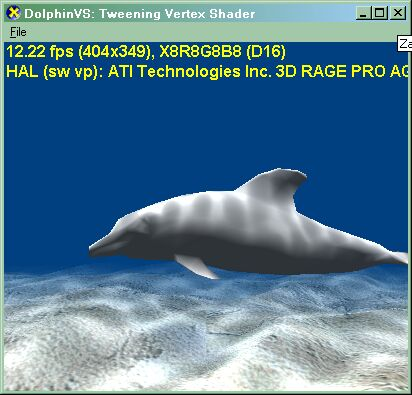
\includegraphics[width=0.75\textwidth]{./pic/dx0}
\caption{Jeden z przykładowych programów z DirectX 9 SDK}
\end{center}
\end{figure}

Programy DirectX.NET mogą być kompilowane zarówno z poziomu środowiska Visual Studio .NET, 
bezpośrednio z linii poleceń ale także z poziomu na przykład Sharp Developa. 
Dla celów kompilacji z linii poleceń przygotujmy prosty skrypt (nazwijmy go {\tt compile.bat}):

\begin{scriptsize}
\begin{verbatim}
csc.exe "/lib:C:\WINNT\Microsoft.NET\Managed DirectX\v4.09.00.0900" 
/r:Microsoft.DirectX.dll %1
\end{verbatim}
\end{scriptsize}

Skrypt ten będziemy wołać z parametrem zawierającym nazwę kompilowanego programu. 
Jeśli kompilowany program będzie wymagał referencji do większej ilości bibliotek, 
wystarczy dodać je jako kolejne parametry.

\subsubsection{Pierwszy program w DirectX.NET}

Pierwszy i najprostszy programem jaki napiszemy będzie tworzył powierzchnię DirectDraw i 
kopiował jej zawartość do okna. Tak naprawdę będzie nam potrzebna jedynie instancja 
obiektu urządzenia DirectDraw oraz obiektu opisującego powierzchnię DirectDraw.

\begin{scriptsize}
\begin{verbatim}
private Device  draw      = null; 
private Surface primary   = null;
\end{verbatim}
\end{scriptsize}

Oba obiekty są tworzone i kojarzone - urządzenie z oknem, a powierzchnia z urządzeniem:

\begin{scriptsize}
\begin{verbatim}
draw = new Device(); 
draw.SetCooperativeLevel(this, CooperativeLevelFlags.Normal);
	. . .
SurfaceDescription description = new SurfaceDescription(); 
description.SurfaceCaps.PrimarySurface = true; 
primary = new Surface(description, draw);
\end{verbatim}
\end{scriptsize}

Ponieważ powierzchnia DirectDraw jest obiektem, wszelkie operacje takie jak rysowanie, 
blokowanie czy zamiana stron są po prostu metodami odpowiedniego obiektu. 
Prosty kształt narysujemy więc za pomocą metody:

\begin{scriptsize}
\begin{verbatim}
primary.DrawCircle( .... );
\end{verbatim}
\end{scriptsize}

a tekst za pomocą metody:

\begin{scriptsize}
\begin{verbatim}
primary.DrawText( ... );	
\end{verbatim}
\end{scriptsize}

Interfejs obiektowy sprawdza się zwłaszcza w przypadku środowisk z autouzupełnianiem kodu - 
tam programista nie musi nawet zaglądać do dokumentacji biblioteki, ponieważ wszystkie metody 
obiektu pojawią się natychmiast po wpisaniu kropki po nazwie obiektu.

Poniższy przykład można bez trudu rozbudować o prostą animację, dodać podwójne buforowanie oraz 
wyświetlanie obrazu na pełnym ekranie. Proponuję potraktować to jako ćwiczenie, zerkając 
w razie potrzeby do przykładów z SDK. 

\begin{scriptsize}
\begin{verbatim}
/* Wiktor Zychla, 2003 */
using System;
using System.Drawing;
using System.ComponentModel;
using System.Windows.Forms;
using Microsoft.DirectX;
using Microsoft.DirectX.DirectDraw;

namespace DirectXTutorial
{
    public class DirectDrawForm : System.Windows.Forms.Form
    {        
        private Device  draw      = null; 
        private Surface primary   = null; 
        private Clipper clip      = null; 

        static void Main() 
        {
          Application.Run(new DirectDrawForm());
        }

        public DirectDrawForm()
        {
           this.ClientSize = new System.Drawing.Size(292, 266);
           this.Name = "DirectDraw w oknie";
           this.Text = "DirectDraw w oknie";
           this.Resize      += new System.EventHandler(this.DDForm_SizeChanged);
           this.SizeChanged += new System.EventHandler(this.DDForm_SizeChanged);
           this.Paint       += 
	     new System.Windows.Forms.PaintEventHandler(this.DDForm_Paint);

           draw = new Device(); 
           draw.SetCooperativeLevel(this, CooperativeLevelFlags.Normal); 
           CreateSurfaces(); 
        }

        private void DDForm_Paint(object sender, System.Windows.Forms.PaintEventArgs e)
        {
           Draw();
        }
        
        private void DDForm_SizeChanged(object sender, System.EventArgs e)
        {
           Draw();
        }
        
        private void Draw()
        {
           if ( primary == null ) return;           
           if ( WindowState == FormWindowState.Minimized ) return;
            			
           Point p = this.PointToScreen( new Point( 0, 0 ) );
           primary.ColorFill( Color.Blue );
           primary.ForeColor = Color.White;
           primary.DrawText( p.X, p.Y, "Pierwszy program w DirectX.NET", false );
        }
                                
        private void CreateSurfaces()
        {
            SurfaceDescription description = new SurfaceDescription(); 

            description.SurfaceCaps.PrimarySurface = true; 
            primary     = new Surface(description, draw); 
            clip        = new Clipper(draw); 
            clip.Window = this; 
            primary.Clipper = clip; 
        }
    }
}
\end{verbatim}
\end{scriptsize}

\subsubsection{Direct3D}

\begin{figure}
\begin{center}
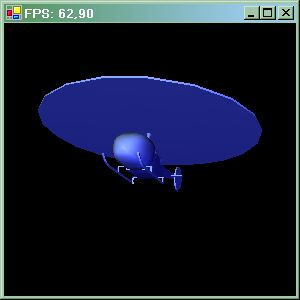
\includegraphics[width=0.50\textwidth]{./pic/dx1}
\caption{Trójwymiarowy świat Direct3D}
\end{center}
\end{figure}

Direct3D jest najciekawszą częścią DirectX.NET. W każdej kolejnej wersji DirectX programiści 
dostają do rąk coraz potężniejsze narzędzia do tworzenia grafiki 3D. W wersji 9 możliwości są 
przeogromne: od tworzenia prostych obiektów, modelowania światła, tekstur, przez manipulację 
siatkami obiektów ({\em vertex shading}) aż do zaawansowanego nakładania tekstur ({\em pixel shading}).  

Aby przekonać się jak sprawuje się obiektowy interfejs Direct3D, napiszemy prosty przykład. 
Z pliku załadujemy opis siatki obiektu 3d ({\em mesh}), dodamy 2 światła, kamerę i na koniec ożywimy 
całość dodając jakiś ruch.

\begin{scriptsize}
\begin{verbatim}
/* Wiktor Zychla, 2003 */
using System;
using System.Drawing;
using System.Windows.Forms;
using Microsoft.DirectX;
using Microsoft.DirectX.Direct3D;

namespace DirectXTutorial
{
  public class DirectXForm : Form 
  {
    Device   device;
    Mesh     mesh;
    int      meshParts = 0;
    Material material;
    float    rotationAngle = 0;
    PresentParameters pp;

    public DirectXForm() 
    {
      this.Size = new Size(300, 300);
      this.Text = "DirectX.NET";
    }

    bool InitializeGraphics() 
    {
      try
      {
        pp = new PresentParameters();
        pp.Windowed = true;
        pp.SwapEffect = SwapEffect.Discard;
        pp.EnableAutoDepthStencil = true;
        pp.AutoDepthStencilFormat = DepthFormat.D16;

        device = new Device(0, DeviceType.Hardware, this, 
	                    CreateFlags.SoftwareVertexProcessing, pp);
        device.DeviceReset += new EventHandler(OnDeviceReset);

        InitializeD3DObjects();

        return true;
      }
      catch (DirectXException)
      {
        return false;
      }
    }

    void InitializeD3DObjects() 
    {
      CreateMesh();
      CreateMaterials();
      CreateLights();
      InitializeView();
    }

    void OnDeviceReset(object o, EventArgs e) 
    {
      InitializeD3DObjects();
    }

    protected override void OnKeyPress(System.Windows.Forms.KeyPressEventArgs e)
    {
      if ((int)(byte)e.KeyChar == (int)Keys.Escape)
        this.Close(); // zakończ 
    }

    void CreateMesh() 
    {
      //mesh = Mesh.Teapot( device );
      //meshParts = 1;

      ExtendedMaterial[] m = null;

      mesh = Mesh.FromFile( "heli.x", 0, device, out m );
      meshParts = m.Length;
    }

    void CreateMaterials() 
    {
      material = new Material();
      material.Ambient = Color.FromArgb( 0, 80, 80, 80);
      material.Diffuse = Color.FromArgb(0, 200, 200, 200);
      material.Specular = Color.FromArgb(0, 255, 255, 255);
      material.SpecularSharpness = 128.0f;
    }

    void CreateLights() 
    {
      Light light0 = device.Lights[0];
      Light light1 = device.Lights[1];

      light0.Type = LightType.Directional;
      light0.Direction = new Vector3(-1, 1, 5);
      light0.Diffuse = Color.Blue;
      light0.Enabled = true;
      light0.Commit();

      light1.Type = LightType.Spot;
      light1.Position  = new Vector3(-10, 10, -50);
      light1.Direction = new Vector3(10, -10, 50);
      light1.InnerConeAngle = 0.5f;
      light1.OuterConeAngle = 1.0f;
      light1.Diffuse        = Color.LightBlue;
      light1.Specular       = Color.White;
      light1.Range          = 1000.0f;
      light1.Falloff        = 1.0f;
      light1.Attenuation0   = 1.0f;
      light1.Enabled        = true;
      light1.Commit();

      device.RenderState.Lighting = true;
      device.RenderState.DitherEnable = false;
      device.RenderState.SpecularEnable = true;
      device.RenderState.Ambient = Color.FromArgb(0, 20, 20, 20);
    }

    void InitializeView() 
    {
      Vector3 eyePosition = new Vector3(0, 0, -20);
      Vector3 direction   = new Vector3(0, 0, 0);
      Vector3 upDirection = new Vector3(0, 1, 0);

      Matrix view = Matrix.LookAtLH(eyePosition, direction, upDirection );
      device.SetTransform(TransformType.View, view);

      float fieldOfView = (float)Math.PI/4;
      float aspectRatio = 1.0f;
      float nearPlane   = 1.0f;
      float farPlane    = 500.0f;

      Matrix projection = Matrix.PerspectiveFovLH(fieldOfView, 
                            aspectRatio, nearPlane, farPlane);
      device.SetTransform(TransformType.Projection, projection);
    }

    void AdvanceFrame() 
    {
      rotationAngle += 0.02f;
      rotationAngle %= Geometry.DegreeToRadian(360);

      Matrix rotateX = Matrix.RotationX(rotationAngle);
      Matrix rotateY = Matrix.RotationY(rotationAngle);
      Matrix world = Matrix.Multiply(rotateX, rotateY);
      device.SetTransform( TransformType.World, world );
    }

    void Render() 
    {
      device.Clear(ClearFlags.Target | ClearFlags.ZBuffer, 
                   Color.Black.ToArgb(), 1.0f, 0);
      device.BeginScene();
      device.Material = material;

      for ( int i=0; i<meshParts; i++ )
        mesh.DrawSubset(i);

      device.EndScene();
      device.Present();
    }

    public static void Main() 
    {
      using ( DirectXForm dxForm = new DirectXForm() )
      {
        if (!dxForm.InitializeGraphics()) 
        {
          MessageBox.Show( "Błąd inicjowania Direct3D." );
          return;
        }
			
        dxForm.Show();

        DateTime start = DateTime.Now;
        int      frame = 0;
        while ( dxForm.Created )
        {
          frame++;
          dxForm.AdvanceFrame();
          dxForm.Render();

          dxForm.Text = String.Format( "FPS: {0:N}", 
	             frame/((TimeSpan)(DateTime.Now-start)).TotalSeconds );
          Application.DoEvents();
        }
      }
    }
  }
}
\end{verbatim}
\end{scriptsize}
 
Przyjrzyjmy się przykładowemu fragmentowi, który tworzy macierze widoku i perspektywy i po 
raz kolejny zwróćmy uwagę jak elegancko spisuje się tutaj model obiektowy DirectX.NET:

\begin{scriptsize}
\begin{verbatim}
Vector3 eyePosition = new Vector3(0, 0, -20);
Vector3 direction   = new Vector3(0, 0, 0);
Vector3 upDirection = new Vector3(0, 1, 0);
Matrix view = Matrix.LookAtLH(eyePosition, direction, upDirection );
device.SetTransform(TransformType.View, view);
float fieldOfView = (float)Math.PI/4;
float aspectRatio = 1.0f;
float nearPlane   = 1.0f;
float farPlane    = 500.0f;
Matrix projection = Matrix.PerspectiveFovLH(fieldOfView, aspectRatio, 
  nearPlane, farPlane);
device.SetTransform(TransformType.Projection, projection);
\end{verbatim}
\end{scriptsize}

Na uwagę zasługuje także nieco inna niż w typowej aplikacji okienkowej konstrukcja pętli głównej programu, 
dzięki której uzyskuje się maksymalną możliwą wydajność animacji. 

Otóż w zwykłej aplikacji okienkowej w C\# w funkcji Main pisze się najczęściej po prostu:

\begin{scriptsize}
\begin{verbatim}
Application.Run( new fMain() );
\end{verbatim}
\end{scriptsize}

Jednak przy takiej konstrukcji aby uzyskać jakikolwiek ruch musielibyśmy utworzyć zegar, 
ustawić go na jakiś kwant czasu i podczas obsługi zdarzenia zegara tworzyć kolejną ramkę animacji. 
Takie rozwiązanie ma dużą wadę: zakładamy bowiem że kwant czasu zaprogramowanego zegara odpowiada mniej 
więcej możliwości tworzenia płynnego obrazu przez maszynę. O wiele lepiej byłoby tworzyć obraz 
natychmiast po tym, kiedy skończy się tworzenie poprzedniej ramki. 

W pierwszej chwili wydaje się, że wymagałoby to zejścia aż na poziom pętli obsługi komunikatów, 
jednak nieoczekiwane, jest to możliwe w C\# na poziomie kodu obiektowego:

\label{netPetlaObslugiKomunikatow}

\begin{scriptsize}
\begin{verbatim}
using ( DirectXForm dxForm = new DirectXForm() )
{
  . . .			
  dxForm.Show();
  . . .
  while ( dxForm.Created )
  {
    dxForm.AdvanceFrame();
    dxForm.Render();

    Application.DoEvents();
  }
}
\end{verbatim}
\end{scriptsize}

Podobnie jak w przypadku DirectDraw, proponuję ten prosty przykład potraktować jako szablon do 
dalszych eksperymentów. 

